The aim of this chapter is to show the characteristics of new detectors to be used as part of the ATLAS experiment
upgrade,
and how to achieve the requirements of the high luminosity operation.
The results of each test to characterize the detector are presented in this chapter.


\section{High Luminosity Large Hadron Collider}

The Large Hadron Collider (LHC), located at the European Organization for Nuclear Research (CERN, derived from {\it Conseil
Europ\'een pour la Recherche Nucl\'eaire}) at the Franco-Swiss border near Geneva is a circular accelerator of 27km
circunference of
acceleration pipes, constitues the largest scientific instrument ever designed and built for scientific research.  It has been
successfully commissioned in March 2010 for proton-proton collision with a \SI{7}{GeV} center-of-mass energy.\par

The LHC is pushing the limits of human knowledge, enabling physicists to go beyond the Standard Model (SM): the
enigmatic Higgs boson, the mysterious Dark Matter and the world of super symmetry are just three of the long-awaited
mysteries that the LHC is working to unveil. \par

The announcement given by CERN on 4 July 2012 about the discovery of a new boson at 125-126GeV\cite{atlas,cms}, almost
certainly the long awaited Higgs particle, is the first fundamental discovery, hopefully the first of a series, that the
LHC can deliver.\\ Such discovery was made possible thanks to the general-purpose detectors ATLAS and CMS, both located
at 2 interaction regions, complemented by the specialized detectors ALICE and LHCb.




% -------- LHC Schedule Table ------ 
\begin{center}
\begin{table}[H]\footnotesize
\centering
\begin{tabular*}{0.8\textwidth}{rcccc}
\cellcolor{blue} &\cellcolor{blue}\textcolor{white}{Period} &\cellcolor{blue}\textcolor{white}{Energy $\sqrt{s}$} &\cellcolor{blue}\textcolor{white}{Luminosity ${\cal
L}$} &\cellcolor{blue}\textcolor{white}{Integrate ${\cal L}$} \\
\cellcolor{cyan} \textcolor{white}{Run I} 	& 2010-2012 & 7-8 TeV & \SI{6e33}{cm^{-2}s^{-1}} & \SI{25}{fb^{-1}}\\
\cellcolor{cyan} \textcolor{white}{LS1} 		&\cellcolor{lightgray}2013-2014 &
\multicolumn{3}{l}{\cellcolor{lightgray}LHC: Go to design energy, nominal luminosity,
bunch spacing 25ns}\\
\cellcolor{cyan} \textcolor{white}{Phase 0} & 2015-2018 & 14 TeV & \SI{1e34}{cm^{-2}s^{-1}} & \SIrange{75}{100}{fb^{-1}}\\
\cellcolor{cyan} \textcolor{white}{LS2} 		&\cellcolor{lightgray}2019-2020 &
\multicolumn{3}{l}{\cellcolor{lightgray}ATLAS: Upgrade $\mu$ spectrometer;NSW,LAr
Calorimeter \& FTK}\\
\cellcolor{cyan} \textcolor{white}{Phase 1} & 2021-2023 & 14 TeV & \SI{2e34}{cm^{-2}s^{-1}} & $\sim$\SI{350}{ fb^{-1}}\\
\cellcolor{cyan} \textcolor{white}{LS3} 		&\cellcolor{lightgray}2024-2025 &
\multicolumn{3}{l}{\cellcolor{lightgray}ATLAS: New Inner Tracker and trigger
architecture}\\
\cellcolor{cyan} \textcolor{white}{Phase 2} & 2026-2030 & 14 TeV & \SI{5e34}{cm^{-2}s^{-1}} & $\sim$\SI{3000}{fb^{-1}}\\
\end{tabular*}
\caption{LHC Schedule \& upgrades for ATLAS detector.}\label{lhcschedule}
\end{table}
\end{center}
The LHC baseline programme until 2030 is shown in Table \ref{lhcschedule}. After entering into the nominal energy regime
of \SIrange{13}{14}{TeV} centro-fo-mass energy in 2015, it is expected that the LHC will reach the design luminosity of
\SI{1e34}{cm^{-2}s^{-2}}. This peak value should give a total integrated luminosity of about \SI{40}{fb^{-1}} per year.
In the period 2019-2023 the LHC will hopefully further increase to two times the peak luminosity, reaching at the end of
2023 an integrated luminosity of about \SI{350}{fb^{-1}}.\par

After the Long Shutdown 3 (LS3) the machine will be in the High Luminosity configuration (HL-LHC). For its successful
realization, a number of key novel technologies have to be developed, validated, and integrated, accompanied with
upgrades from the
general purpose detectors such as ATLAS.


\section{ATLAS Detector}

The ATLAS detector is a general-purpose experiment, designed to explore proton-proton collisions at center of mass up to
$\sqrt{s}=$14GeV in the Large Hadron Collider (LHC) at the European Laboratory for Particle Physics (CERN). It is aiming
to understand the foundations of matter and forces, in particular the nature of mass in a broad physics program. The
ATLAS detector was built with the ability to discover the Higgs boson over a wide mass range. It can also perform
searches for the production of heavy particles that would indicate physics beyond the Standard Model, such as super
symmetric particles, as well as searches for other massive objects. \par 

The ATLAS experiment includes complex detector systems. The central part is a cylindrical Inner Detector, to detect
charged particles produced in the collisions, and as such, it is a compact and highly sensitive component. It consists of
three different systems of sensors, all immersed in a magnetic field parallel to the beam axis. The {\bf Inner Detector}
measures the direction, momentum, and charge of electrically-charged particles produced in each proton-proton collision.
The next part is the Calorimeter (red and green on figure ~\ref{fig:ATLAS}), which  measures the energy of a particle
when it loses its energy as it passes through the detector. It is usually designed to stop entirely or ``absorb" most of
the particles coming from a collision, forcing them to deposit all of their energy within the detector. Calorimeters
typically consist of layers of ``passive" or ``absorbing" high-dense material -for example, lead-interleaved with layers
of an ``active" medium such as scintillator or liquid argon.\par
Electromagnetic calorimeters measure the energy of electrons and photons as they interact with matter. Hadronic
calorimeters sample the energy of hadrons (particles that contain quarks, such as protons and neutrons) as they interact
with atomic nuclei. The components of the ATLAS calorimetry system are: the {\bf Liquid Argon (LAr) Calorimeter} and the
{\bf Tile Hadronic Calorimeter}.\par
\begin{figure}[H]
		\centering
		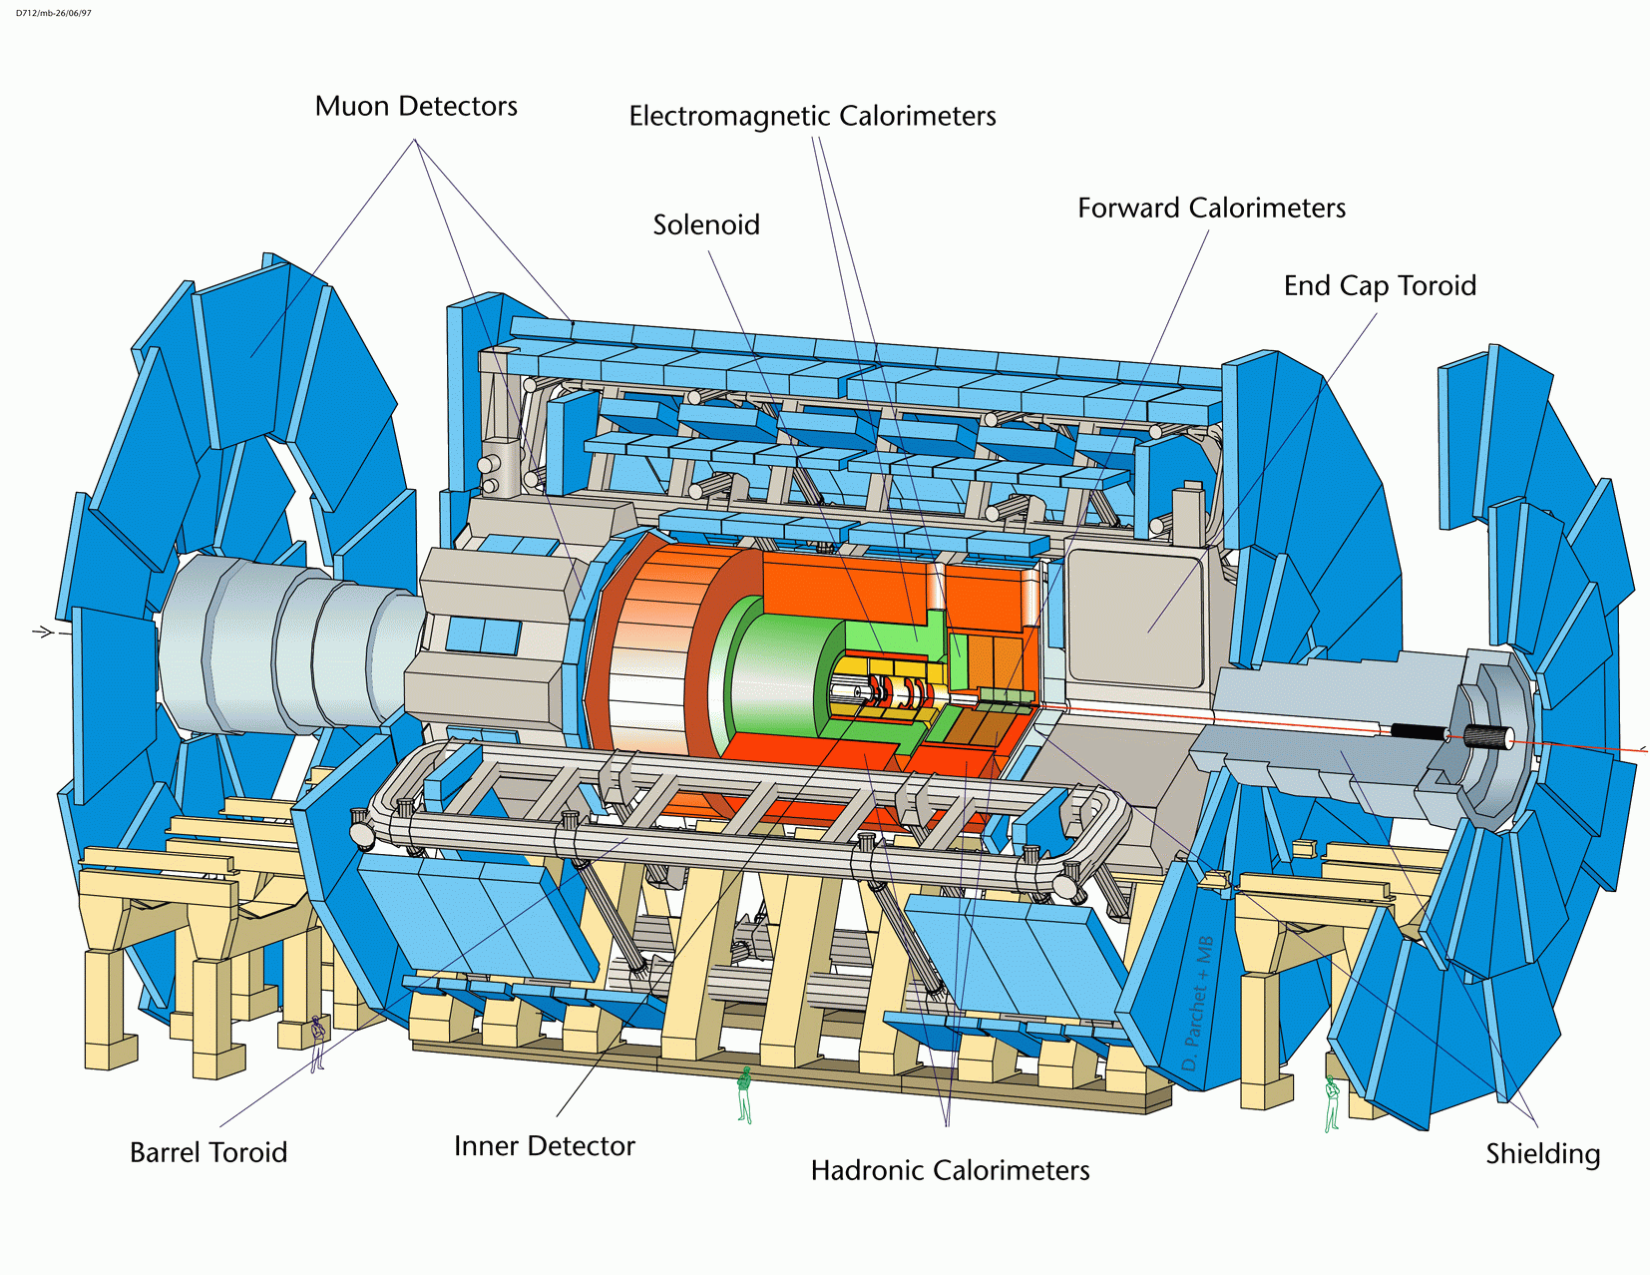
\includegraphics[width=0.6\textwidth]{ATLAS.pdf}
		\caption{ATLAS detector, Muon Spectrometer (in blue)}\label{fig:ATLAS}
\end{figure}

Calorimeters can stop most known particles except muons and neutrinos. Muons are charged particles that pass through the
Inner Detector and Calorimeter interacting only by ionization, they can penetrate through large amount of material without any strong
interaction, they have long lifetime, therefore, can be considered as stable particles within the detector's volume, and
provide a good tagging for the lepton's decays channels.\par

To trigger and detect these particles, the ATLAS experiment uses the {\bf Muon Spectrometer}, made up of 4.000
individual muon chambers (different types of gas chambers) which are in charge of identify each one of these muons. It
is only possible to measure their momentum with the help of the {\bf Magnet System}, made of three sections; the {\bf
Central Solenoid Magnet} with a 2T magnetic field that bends the charged particles for momentum measurement near the
interaction points, helping the Inner Tracker system, the {\bf Barrel Toroid} bends the muon particles in the low
rapidity region, and the {\bf Endcap Toroid} with a 4T magnetic field that bends the muons in the high rapidity
region.\par
% -------------------------------------- Coordinate system -------------------------------------- 
\subsection{Coordinate system}

A common coordinate system is used through ATLAS. The interaction point is defined as the origin of the coordinate
system. The z-axis runs along the beam line. The x-y plane is perpendicular to the beam line and is referred to as the
transverse momentum, $p_T$. The positive x-axis points from the interaction point to the center of the LHC ring; the
positive y-axis points upward to the surface of the earth. The detector which is located half at positive z-values is
referred to as the ``A-side'', to the other half the ``C-side''. The transverse plane is often described in terms of
$r-\phi$ coordinates. The azimuthal angle $\phi$ is measured from the x-axis, around the beam. The radial dimension,
$r$, measures the distance from the beam line. The polar angle $\theta$ is defined as the angle from the positive
z-axis. The polar angle is often reported in terms of pseudorapidity, defined as $\eta = -\ln \tan (\theta/2)$. The
distances $\Delta R$ is defined in $\eta-\phi$ space as $\Delta R = \sqrt{\Delta \eta^2 + \Delta \phi^2}$.\par




%\textcolor{red}{Such energy has been achived from 2015 and successfuly working with a
%luminosity of $\mathcal{L}=$\SI{1e34}{cm^{-2}s^{-1}} from 2016.}\\
%\subsubsection{}

\subsection{Detector Upgrade}

To fulfill the LHC program (in table \ref{lhcschedule}), and in order to benefit from the expected high luminosity
performance that will be provided by the Phase-I upgraded LHC, the first station of ATLAS muon end-cap system (Small
Wheel, SW) will need to be replaced.  The {\bf New Small Wheel (NSW)} will have to operate in a high background
providing a radiation region (up to \SI{15}{kHz/cm^2} of photons, and \SI{75}{Hz/cm^2} of neutrons is expected) while
reconstructing muon tracks with high precision as well as furnishing information for the Level-1 trigger. These
performance criteria are demanding. In particular, the precision reconstruction of tracks for offline analysis requires
a spatial resolution of about 100\micro{m}, and the Level-1 trigger track segments have to be reconstructed online with
an angular resolution of approximately 1mrad. \par
\begin{figure}[ht]
		\centering
		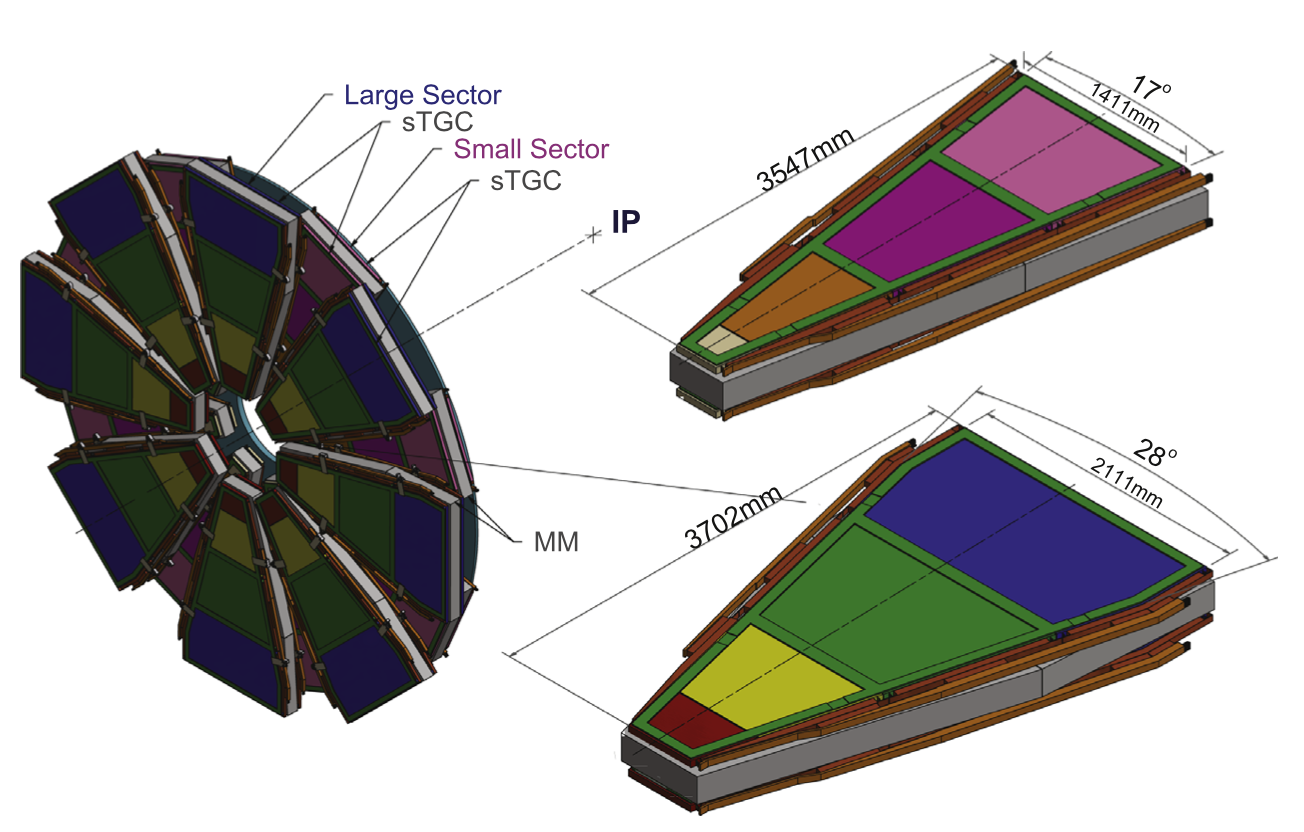
\includegraphics[width=0.7\textwidth]{NSW.png}
		\caption{New Small Wheel}\label{fig:nsw}
\end{figure}

The NSW will have two chamber technologies, one primarily devoted to the Level-1 trigger function (Small-strip Thin Gap
Chambers, sTGC) and the other one dedicated to precision tracking (Micromegas detectors, MM). The sTGC is deployed for
triggering given their single bunch crossing identification capability, a fast response and good position
resolution.\par

The MM detectors have exceptional precision tracking capabilities due to their small gap (\unit{5}{mm}) and strip pitch
(approximately 0.5\si{mm}). Such a precision is crucial to maintain the current ATLAS muon momentum resolution in the
high background environment of the upgraded LHC.  The MM chambers can, at the same time, confirm the existence of track
segments found by the muon end-cap middle station (Big Wheels) online. The sTGC has the additional ability to measure
offline muon tracks with good precision, so the sTGC-MM chamber technology combination forms a fully redundant detector
system for triggering and tracking both for online and offline functions. This detector combination has been designed to
be able to provide excellent performance for the eventual High Luminosity LHC upgrade.\par 



\section{sTGC Description}

The small-strip Thin Gap Chamber (a.k.a sTGC) is a multi-wire proportional chamber (MWPC), a detector type with a
relatively old technology. Its successful introduction to detector systems in 1968 has earned eGeorges Charpak the Nobel
prize in Physics 1992.  Those devices have been a major ingredient to detector systems since they can achieve spatial
resolution of tenths microns, and have typical time resolution of about 50ns.\par

The sTGC has been design to exploit these features,  working with a cathode-anode pitch smaller than the anode-anode pitch, mostly based on the design of
the Thin Gap Chamber\cite{tgc}, with thinner strips as the main improvement from the previous version. The TGC
technology has been used since 1988 in the OPAL experiment\cite{opal} and is currently part of the muon spectrometer in ATLAS. \par

This new chamber has the advantage of having a \unit{3.2}{mm} strip-pitch 
compared with the \unit{6}{mm} from the previous TGC, which explains the {\it small-strip} prefix.\par 

Chambers with different strips sizes were built and tested under pion beams, and the \unit{3.2}{mm} pitch was chosen as the best
option to provide a resolution better than \unit{100}{\micro m}\cite{stripwidth}.  This change will improve the
measurement of charge centroid position by charge interpolation.\par To improve the time response, the cathode surface
resistivity has been reduced by a factor 10, to reduce charge accumulations on the cathode when chamber operates at high
rate, lowering from 1 M$\Omega/\square$ to 100-200k$\Omega / \square$ resistivity on the graphite layer.  At the same
time, cathode-readout plane (strips or pads) distance was reduced to \unit{0.1}{mm}(\unit{1.6}{mm} before) to increase
the capacitive coupling by 10, therefore the $RC$ factor keeps unchanged.\par

%----------- sTGC mode picture -----

\begin{figure}[ht]
		\centering
		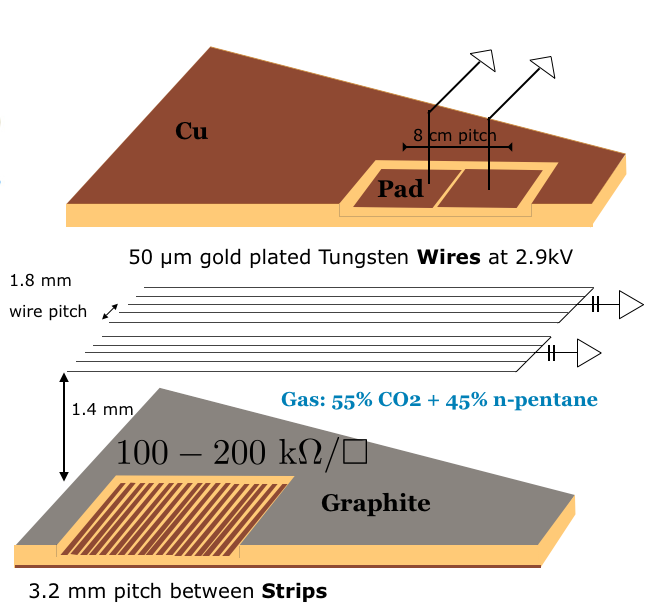
\includegraphics[width=0.5\textwidth]{sTGC_layout.png}
		\caption{Single plane sTGC}\label{fig:sTGC}
\end{figure}

The sTGC is made of two resistive cathodes planes, with copper readout plane with strips on one layer and the other one
with pads, with \unit{8x12}{cm$^2$} area used for fast pattern recognition of tracks to select strips for read out. This
represents a big
advantage compared to the TGC, which does not have this feature.\par

The cathodes are made of FR4 with \unit{1.4}{mm} of thickness, where \si{17}{\micro m} of copper is etched for strips
(pads), pressed with a \unit{100}{\micro m} of FR4 over it and then sprayed with graphite to provide superficial
resistivity.\par

The anodes are golden tungsten wires of \unit{50}{\micro m} diameter,
distributed at \unit{1.8}{mm} of distance between each other and a gas gap of \unit{2.8}{mm}. To work with such geometry, several
tests were made to find the proper gas
mixture\cite{gaschoice}. The most suitable mixture has been found to be 55\% (CO$_2$)
and a quenching gas, a primary ingredient is 45\% of n-pentane(n-C$_5$H$_{12}$), which allows the chamber to work in a limited
proportional region\cite{driftbook}(see Section 1.2.3). 
The latest ingredient; n-pentane, can absorb UV photons due to its many molecular degree of freedom,
hence preventing the chamber from going into a Geiger mode.\par 

%----------- How its produce the ionization and drifts  -----



\subsection{Electric field simulation}

Motivated by gaining better understanding of the detector operational mechanisms, dedicated simulations studies using
gaseous detector simulation tools have been performed. The main simulation tool used is Garfield
\cite{garfield2,garfield1} software package. This set of libraries allows to calculate the electrical field with
geometrical configuration as drift chambers.\par
The simulation uses a coordinate system where x is along the strips, y defines the chamber depth and z is along the
wires.\par

\begin{figure}[ht]
	\centering
	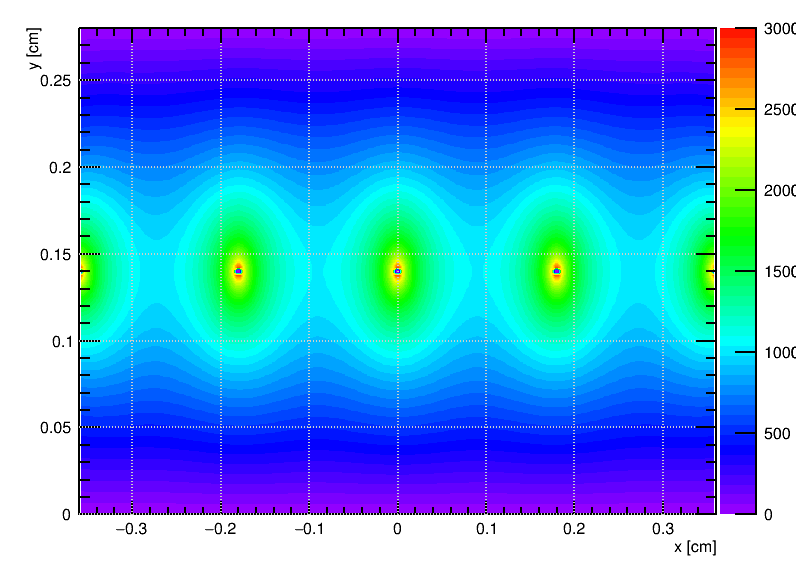
\includegraphics[width=0.5\textwidth]{vfield.png}
	\caption{Equipontential lines, anode at 2900V}\label{fig:vfield}
\end{figure}

\begin{figure}[ht]
		\centering
		\hspace*{\fill}
		\begin{subfigure}[b]{0.45\textwidth}
			\centering
			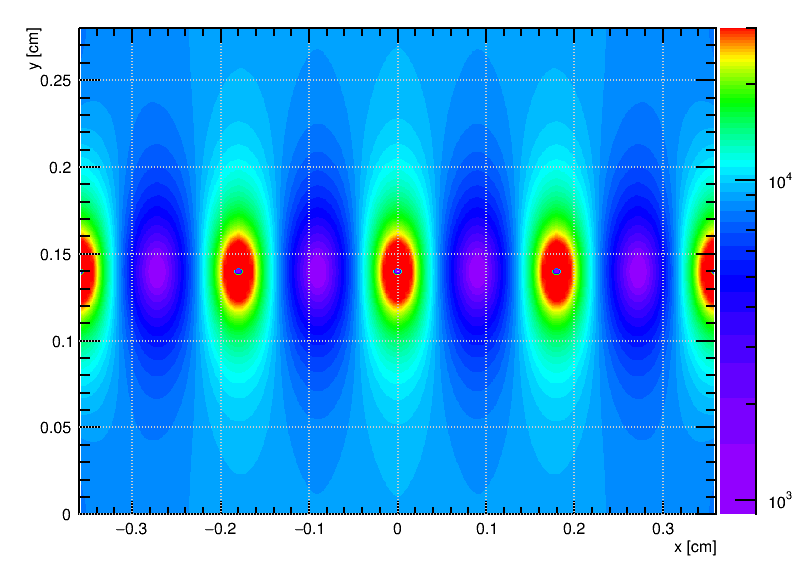
\includegraphics[width=\textwidth]{25efield.png}
			\caption{Electrical field, anodes at 2500V}\label{fig:25efield}
		\end{subfigure}
		\hfill
		\begin{subfigure}[b]{0.45\textwidth}
			\centering
			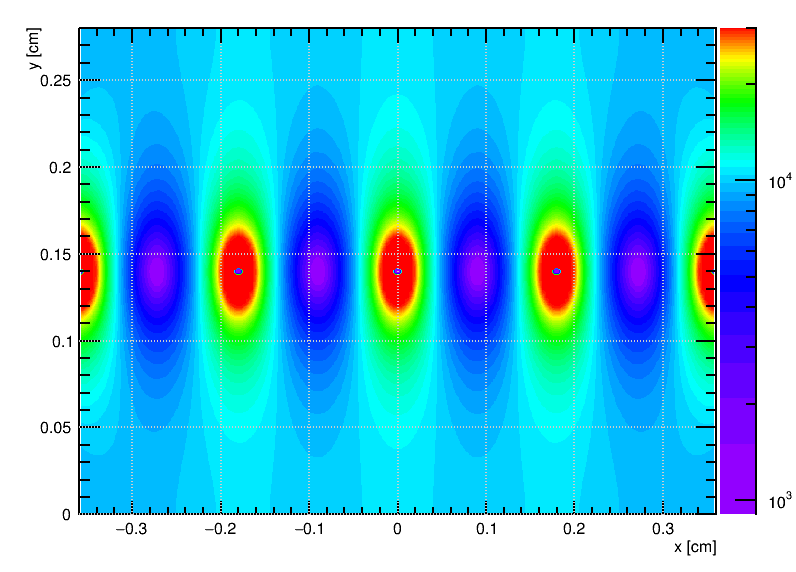
\includegraphics[width=\textwidth]{efield.png}
			\caption{Electrical field, anodes at 2900V}\label{fig:efield}
		\end{subfigure}
		\hspace*{\fill}
		\centering
		\captionsetup{margin=1cm}
		\caption{The electric field map in the x-y plane for a typical operating high voltage 2900V and 2500V.}\label{fig:efields}
\end{figure}

Both contour plots on figure \ref{fig:efields} represent the magnitude of the electrical field with scale of
\SIrange{1e3}{1e5}{V/cm} with 50 steps. At the working potential \SI{2.9}{kV}, it is possible to observed a field
strength of  more than \SI{1e4}{V/cm} over a 97\% of the gas gap. The weakest field is only in a small region in the
middle of two neighboring wires, leading to less than 5\% of long drifting electrons. 


\section{Construction process}

The main novelty on this detector is the high resolution obtained on x-axis due to the strip boards and the alignment
between each chamber to get precision of about 50\micro m and 30\micro m respectively.\par 

It is important to discuss the process which makes it possible to achieve these numbers. Everything relies on how well
these chambers are built and also how the cathodes
boards (strips and pads) are fabricated.\par 

The size of each chamber varies from \SIrange{0.7}{2.5}{m^2} with around 1m long, where over 300-400 strips must be
etched with a precision of 50\micro m. A standard length for printed circuit boards (PCB) is \SI{70}{cm}.  Extremely
precautions must be taken to provide the precision and parallelism between each strips, in one of the biggest PCB board
ever made.\par

The attempt of this section is to provide an overview of how the sTGC Quadruplets are built, mostly on the first module 0
produced by UTFSM, which is the QS1 (Quadruplet Small sector, part 1).  Being the smallest detector to be produced for
the NSW has some pros and cons. The main cons is related to the position of the QS1 inside the NSW; it is the closest
one to the interaction point and as such, it gets the highest rate of particles. For the same reason, the position
resolution is a key point and the high efficiency response under a high rate environment is a must.\par


Some pros are related to its size; with approximately \SI{1.3}{m} long, \SI{35}{cm} the small base and 75cm the large
one of the trapezoidal shape, the sTGC QS1 can be handled without any problems during its construction.\par

\subsubsection{Quality Control of cathode boards}

The cathodes for the module 0 were made by an Italian company MDT, and since it was the first production, the review was
done on-site.\par

The thickness of the board is measured in 19 points around the perimeter with a micrometer. The values of theses
measurements must be within 1.5mm$\pm$25\micro m. Exceeding this numbers leads to the partial rejection of the cathode
boards, however if there is a single point deviation of less than 35\micro m from the average, it could be used in
combination with another cathode board that does not have the same local deviation.\par 
An electrical test is done with a multimeter, to check if there is any short circuit between strips or pads depending on
the cathode board.\par

The last step and the most important is the dimensional control; it is performed on a granite table, with 2 pins that
match the brass inserts on the cathode and a special caliper. 

An aluminum-ruler (Al-ruler) machined (see Figure \ref{fig:ruler}) with a precision of 30\micro m at 20 Celsius degrees is used as
caliper.  Above the cathode board the misalignment is measured. It has the same strip pitch for the first and the last five
strips as well as two intermediate regions, and to avoid any parallax, the thickness of the edge for these strips is 1mm.
Looking with a magnifying glass around 4 regions allows to detect some misalignment between theses strips (caliper
and cathode board). A photography is taken and analyzed to calculate this misalignment. For such distance (about 1 m
long) some precautions must be taken, considering the expansion coefficient for both material.\par
\vspace{1cm}
%------- Photography strip cathode board measurement ------------ % 
\begin{figure}[ht]
	\centering
	\hspace*{\fill}
	{\begin{subfigure}[b]{0.35\textwidth}
		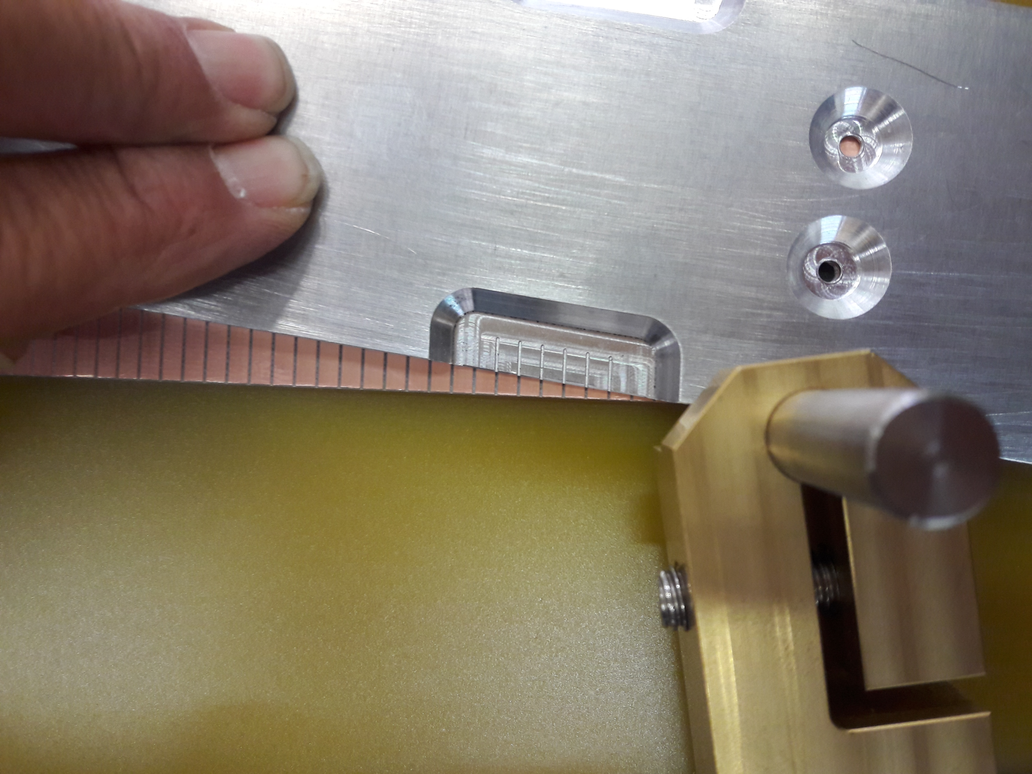
\includegraphics[width=\textwidth]{alignment.png}
		\caption{Al-ruler used to check shift over the last strips.}
		\label{fig:ruler}
	\end{subfigure}
	}
	\hfill
	{\begin{subfigure}[b]{0.35\textwidth}
		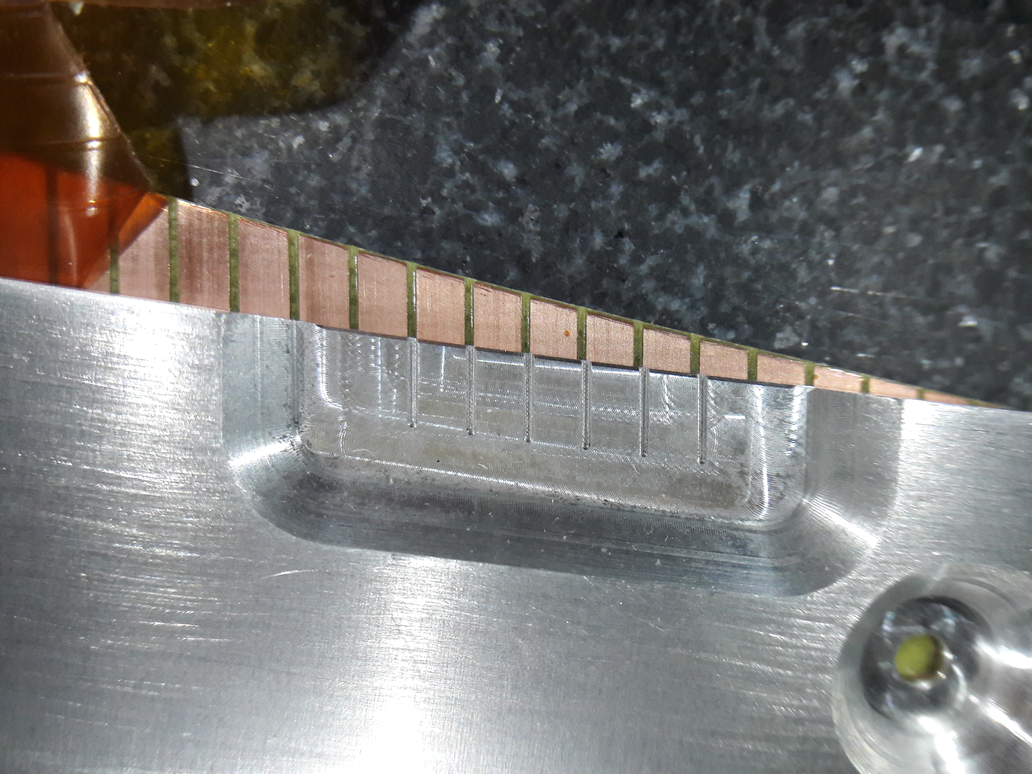
\includegraphics[width=\textwidth]{zoom_in.png}
		\caption{Zoom-in Comparing strip position}
		\label{fig:zoom}
	\end{subfigure}
	}
	\hspace*{\fill}
	\caption{Strip control with {\bf Al} ruler}
\end{figure}

\subsubsection{Cathode preparation}

Once the cathodes pass all the dimensional control, they have to be cleaned with Acetone and Isopropyl alcohol and placed on a
granite table (with a flatness  better than 30\micro m) with a vacuum system underneath. They have to be fixed on the edges with
metal jigs which have marks for the internal wire support or chamber division.\par
The places which are not sprayed with graphite, like the wire support and the edges, are covered with a \unit{3.5}{mm}
black tape on the designated wire support locations across the board. To prevent spraying graphite on the places where
there will be glue, a blue tape must be placed on the edges.

\subsubsection{Graphite spraying}

A key point for this process is to prepare the ``painting", a mixture of Graphite-33 with Plastik-70 bonding agent.\par

The graphite must be agitated for at least 2 hours before mixing with Plastik-70. A proper ratio of 1500g Graphite and
540g Plastik is mixed during 2 hours before spraying.\par

A spraying machine is in charge of this process, and meanwhile temperature and humidity must be controlled.  After the
cathode is painted, the superficial resistivity is measured on the edges. Values must exceed
\unit{100}{k$\Omega/\square$} otherwise the cathode needs to be sprayed again.\par


\subsubsection{Polishing}

In order to ensure an homogeneous resistivity across the chamber, the cathode is visually divided in to 5x6 sections. Inside
each section, the resistivity is measured on 5 to 7 points with a probe. Simultaneously the cathode is brushed in the
same orientation as the wires. The brush must be done carefully, without over-polishing areas, because once the resistance
drops down, nothing will bring it back up. 


\subsubsection{Gluing internal parts}

After removing all the blue and black tapes, all the internal parts (buttons, wire support, etc.) are glued to provide
mechanical support to the anode wires.\par
The wire support and the buttons help the chamber not to bend due to gravity and not to create a catenary effect.
The external frames provide the \unit{1.4}{mm} height for the gas gap. 
All these part are cleaned with isopropyl alcohol, 
While the glue, a type of epoxy (2011-Araldite) is prepared, all these parts are cleaned with isopropyl alcohol.
This glue will not only fix the parts, it will also fill the surfaces where these parts are less thick than requested.


\subsubsection{Winding wires}
A flat table which can spin around one axis is used to wind the cathodes board.
On each side of the table, one cathode with all the internal parts is tight with metal clamps on
the edges. 
At the same time, vacuum is applied underneath to ensure the flatness of the cathode. 
A winding machine places each wire at \unit{1.8}{mm} distance from each other with
\unit{50}{\micro m} precision.\\ 
After the process is completed, all the wires are soldered in batches of 10
over the wire-rulers. The remaining wire can be cut and the HV resistors (10\si{\mega\ohm}) soldered. The metal
clamps around the edges are then removed, and the relative wire tension is checked by comparing the deflection of
adjacent wires.\par

\subsubsection{Detector Assembly}

Once the cathodes are winded and all wires are soldered, the Pad cathode board is cleaned with clean water and dried
with clean air.  The board is placed on the granite table (with vacuum underneath) to be tested with high voltage.  It
is necessary to monitor the current from the cathode while the voltage is increased.  It starts with 100V and reaches
3000V, with steps of  100V.  The current should never reach a value higher than \unit{1}{\micro A}. If it does, the
cathode needs to be checked carefully, to remove dust or glue which create sparkles.\par

Reaching the nominal current, the strip cathode board is placed against the pad cathode board carefully.  An aluminum
frame with a silicon rubber is placed on top to isolate the chamber from the environment.  Afterwards, vacuum is applied
to this chamber and CO$_2$ is flushing inside the chamber.\par 

The power supply is turned on and no sparkles (monitoring the current) must be found.\par 

In order to prevent dust entering the chamber, the glue is prepared to close it immediately.  Upon completion of
the process, a single chamber is built.\par

A doublet is assembled with two single chambers glued with a honeycomb paper. Repeating the process with two doublets,
the quadruplet is built.
\begin{figure}[ht]
\centering
\hspace*{\fill}
{\begin{subfigure}[b]{0.55\textwidth}
\includegraphics[width=\textwidth]{quadreal.png}
\caption{Module \#0 against alignment pin}\label{}
\end{subfigure}
}\hfill
{\begin{subfigure}[b]{0.35\textwidth}
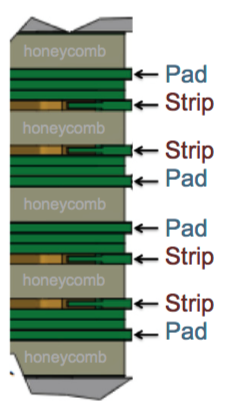
\includegraphics[height=7cm]{quadlayers.png}
\caption{Layer description}\label{quad}
\end{subfigure}
}\hspace*{\fill}
\caption{}
\end{figure}


\section{Gain uniformity measurements}

After the chambers are built, it is important to look for any malfunctioning. A primitive test to check the behavior of
the detector is to move a radiation source across the sensitive area, while the current draw is measured from the
power supply.\par

In this test, it is important to understand what can produce variation on the gain. There are two main factor that can
produce gain variations on wire detectors. The first one is the ``nature" gain fluctuations from the charge production
in proportional counters which follow Polya distribution, however it is less pronounced in limited proportional mode such
as sTGC working region.\par

The second one is related to the mechanical tolerances, this part has been very well known for 40 years as it is
presented in
Sauli's book \cite{sauli} about drift chambers from which we can conclude the following:
\begin{itemize}
\item Variations on the wire diameter of about 1\% (fabrication precision) results in a 3\% change on the gain.
\item A \unit{100}{\micro m} difference in the gas gap thickness (\unit{2.7}{mm}) results in about 15\% change on the gain.
\item The effect of a wire displacement of about \unit{100}{$\mu$m}
of a wire plane results in 1\% in the charge of the two adjacent wires which with a gain of $\sim10^6$ will give a
$\sim10\%$ change on the gain.
\end{itemize}

Taking all of this in consideration, it is expected to get a gain variation of less than 20\% in agreement with the
Construction manual\cite{mann}.\par

The amount of current measured from the power supply is considered as gain reference, while the detector is
irradiated with x-rays. The test is performed under two different working points (bias voltage), 2500V (low gain) and
2900V, the operational voltage.\par

%-------- why x ray source ? ----------
For such test the x-ray source is used due to the following advantages:\par
\begin{itemize}[noitemsep, topsep=0pt, parsep=0pt, partopsep=2pt]
	\item Mostly mono-energetic photons.
	\item Variable photon intensity: Limiting the current from the tube from \SIrange{1}{200}{\micro A} can provide different rates.
	\item Variable photon energy: Varying the breaking voltage of electrons inside the x-ray gun from
	\SIrange{10}{50}{kV}.
	\item Different spot size: with a set of collimator it is possible to irradiate area of interest.
\end{itemize}


\subsection{Setup}
To perform such test, a x-ray gun called Mini-X\cite{xgun} from Amptek is used, with silver (Ag) as transmission target and with a
beryllium (Be) end-window.\par

\begin{figure}
	\centering
	\hspace*{\fill}
	{\begin{subfigure}[b]{0.4\textwidth}
	\centering
	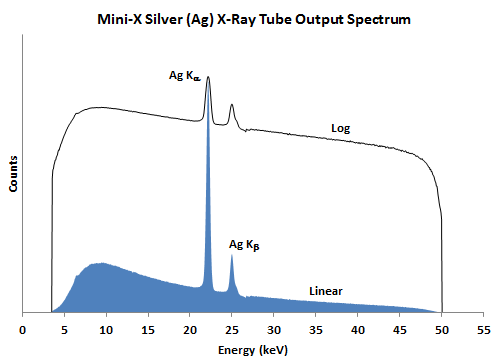
\includegraphics[width=\textwidth]{minix_ag_1.png}
	\caption{Output spectrum, from 0 to 50keV}\label{fig:minixgun}
	\end{subfigure}
	}
	\hfill
	{
	\begin{subfigure}[b]{0.4\textwidth}
	\centering
	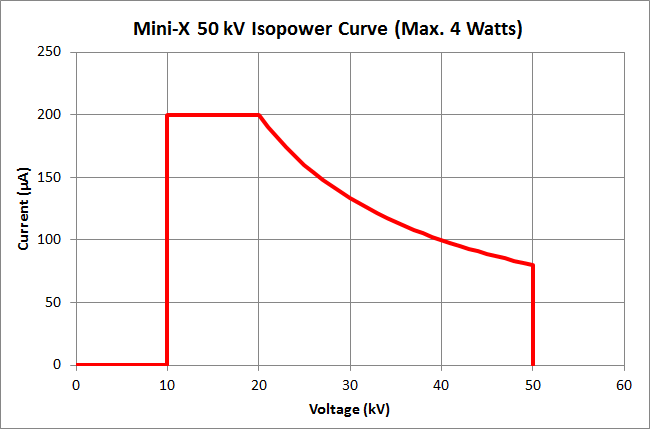
\includegraphics[width=\textwidth]{minix_d.png}
		\caption{Isopower curve for the Mini-x gun}\label{fig:ispower}
	\end{subfigure}
	}
	\hspace*{\fill}
	\caption{}\label{}
\end{figure}

\begin{figure}
	\centering
	\hspace*{\fill}
	{\begin{subfigure}[b]{0.4\textwidth}
	\centering
	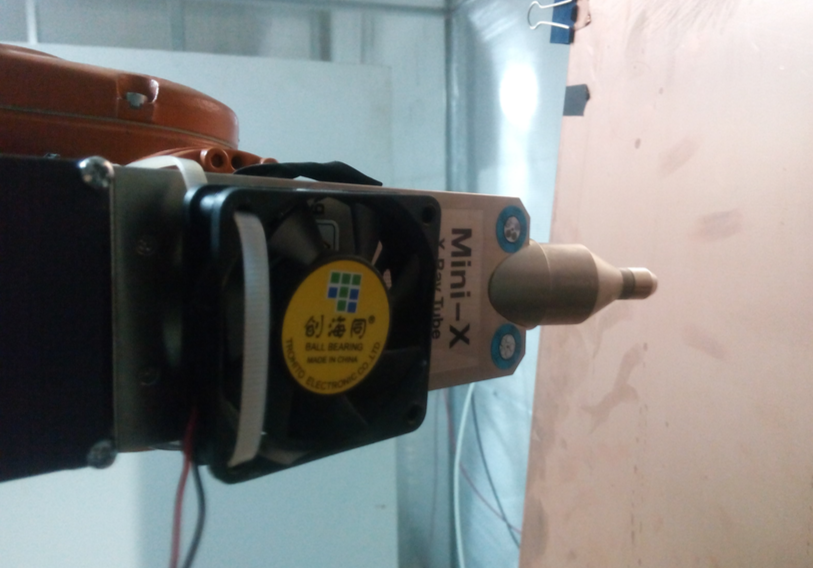
\includegraphics[width=\textwidth]{kuka.png}
	\caption{Mini-X gun mounted on KUKA robo-arm}\label{fig:kuka}
	\end{subfigure}
	}
	\hfill
	{
	\begin{subfigure}[b]{0.4\textwidth}
	\centering
	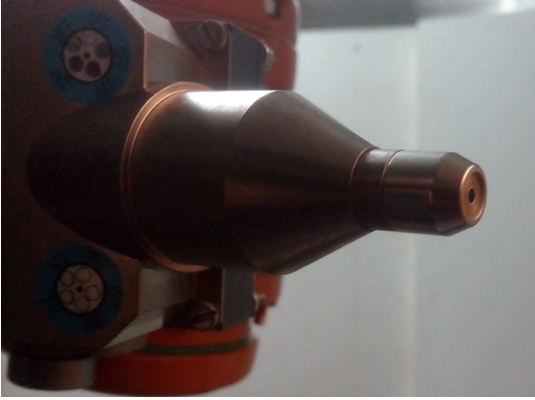
\includegraphics[width=\textwidth]{collimator.png}
		\caption{Collimator 2mm}\label{fig:collimator}
	\end{subfigure}
	}
	\hspace*{\fill}
	\caption{}\label{}
\end{figure}

The gun is mounted on a KUKA robo-arm (see Fig.\ref{fig:kuka}), with a 5 degrees collimator providing a \SI{4}{mm^2}
spot size at a proper distance. The robo-arm provides the x-y movement to scan the whole sensitive detector area, moving
from the small base to the large base along the wires at step of \SI{1.2}{cm/s (y-axis)}.\par

The robo-arm moves along the x-axis in \SI{5}{cm/s} steps.  This is not the most suitable step to irradiate the whole
detector, but it allows the x-ray gun to work properly at \SI{45}{\micro A}, 50keV energy (see figure \ref{fig:ispower})
without overheating.\par

A NIM HV Power Supply Module CAEN 1470 was used to power the chambers. The power supply (PS) was controlled by USB with
the CAEN HV Wrapper Library. The current registered from the PS was written in a ASCII file for further analysis. The
sampling rate used from the PS was 1 per second, giving the current average during this period.  The test is taken in
approximately one hour, irradiating one chamber at the time.\par

Since the detector is already built as a quadruplet, it has to turn over to irradiate its other face. Hence, only
the external layers (chambers) are irradiated directly without having an chamber to provide a screening effect.\par

\begin{figure}[ht]
	\centering
		\hspace*{\fill}
	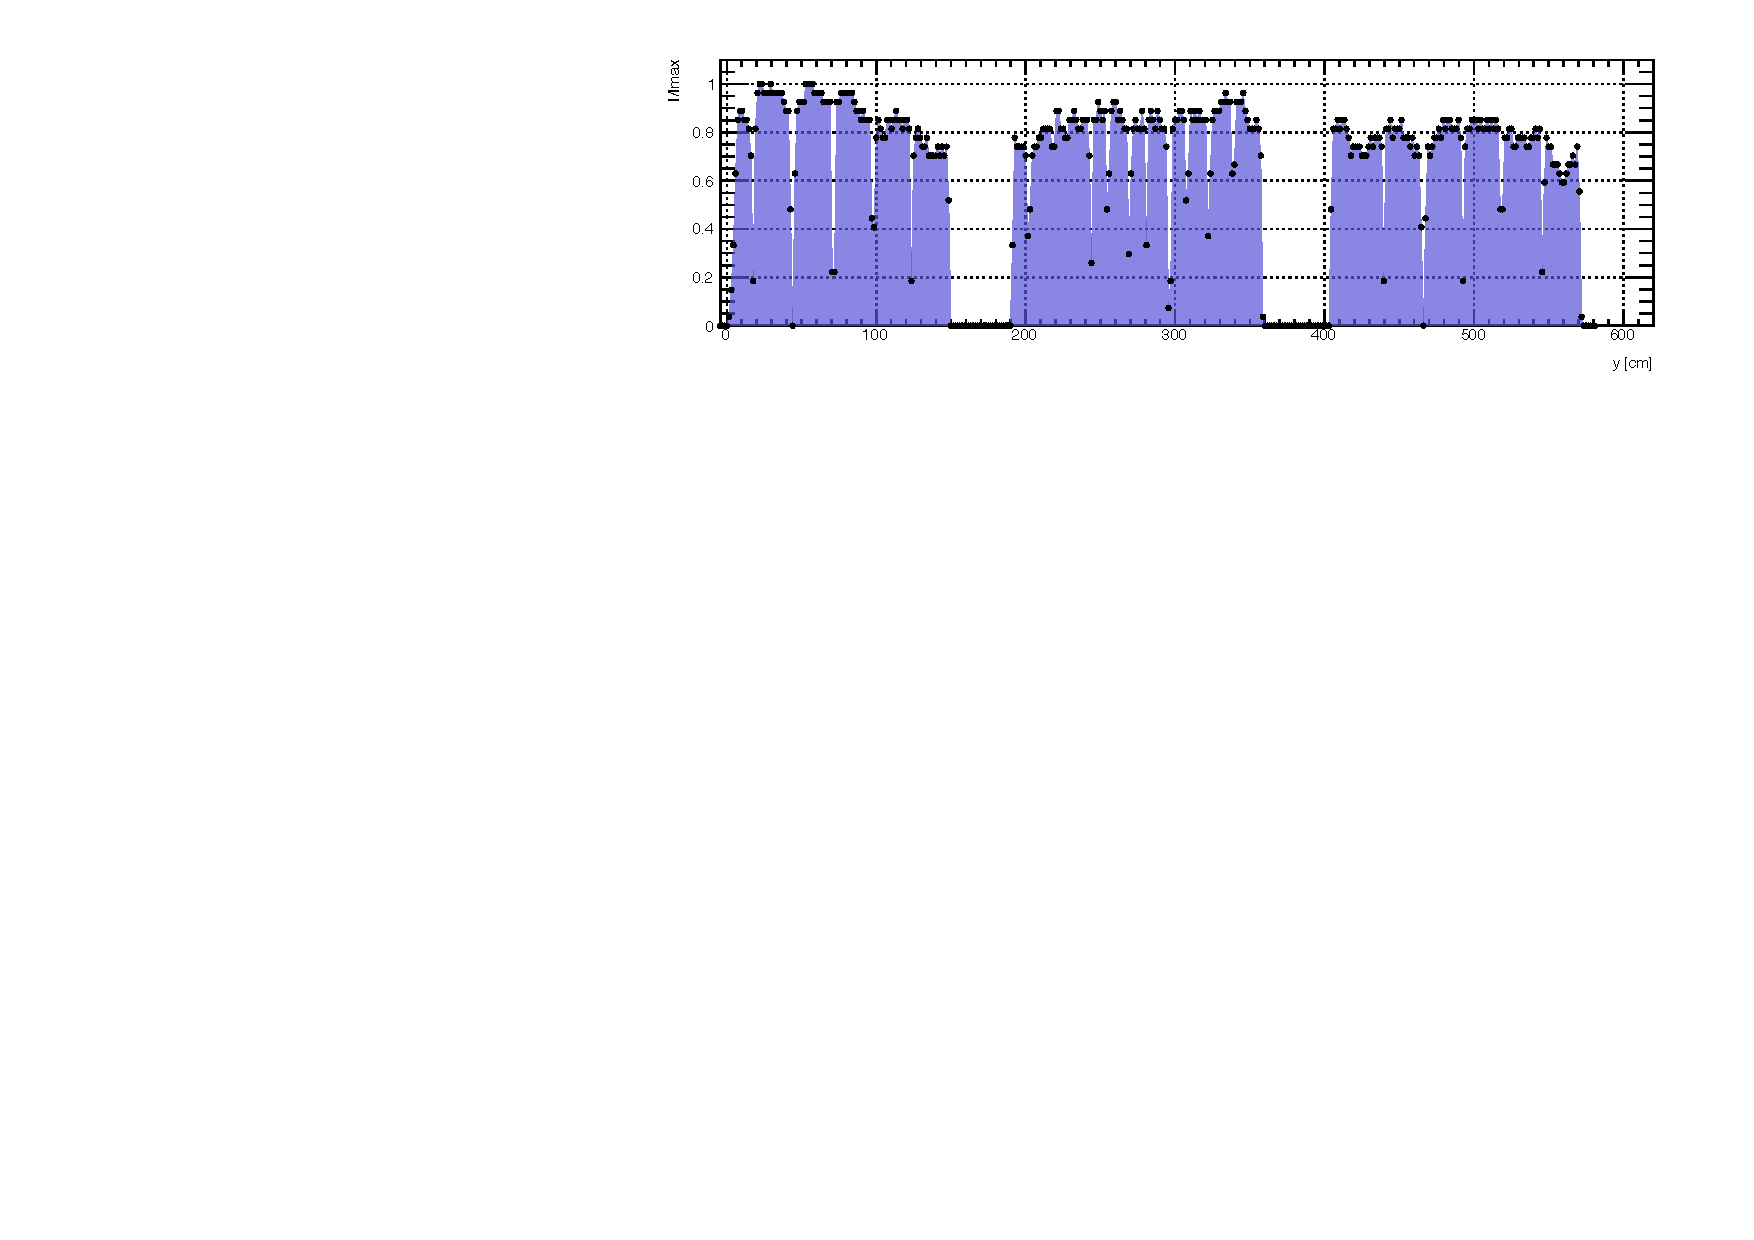
\includegraphics[width=0.9\textwidth]{uniformity_2900.pdf}
		\hspace*{\fill}
		\captionsetup{margin=1cm}
	\caption{Relative current to the maximum, while the robo-arm is moved along the wires. The three set current
	corresponds to the whole detector irradiated in three different positions from x-axis.}\label{}
\end{figure}


\subsection{Results}

\begin{figure}[ht]
	\centering
		\hspace*{\fill}
	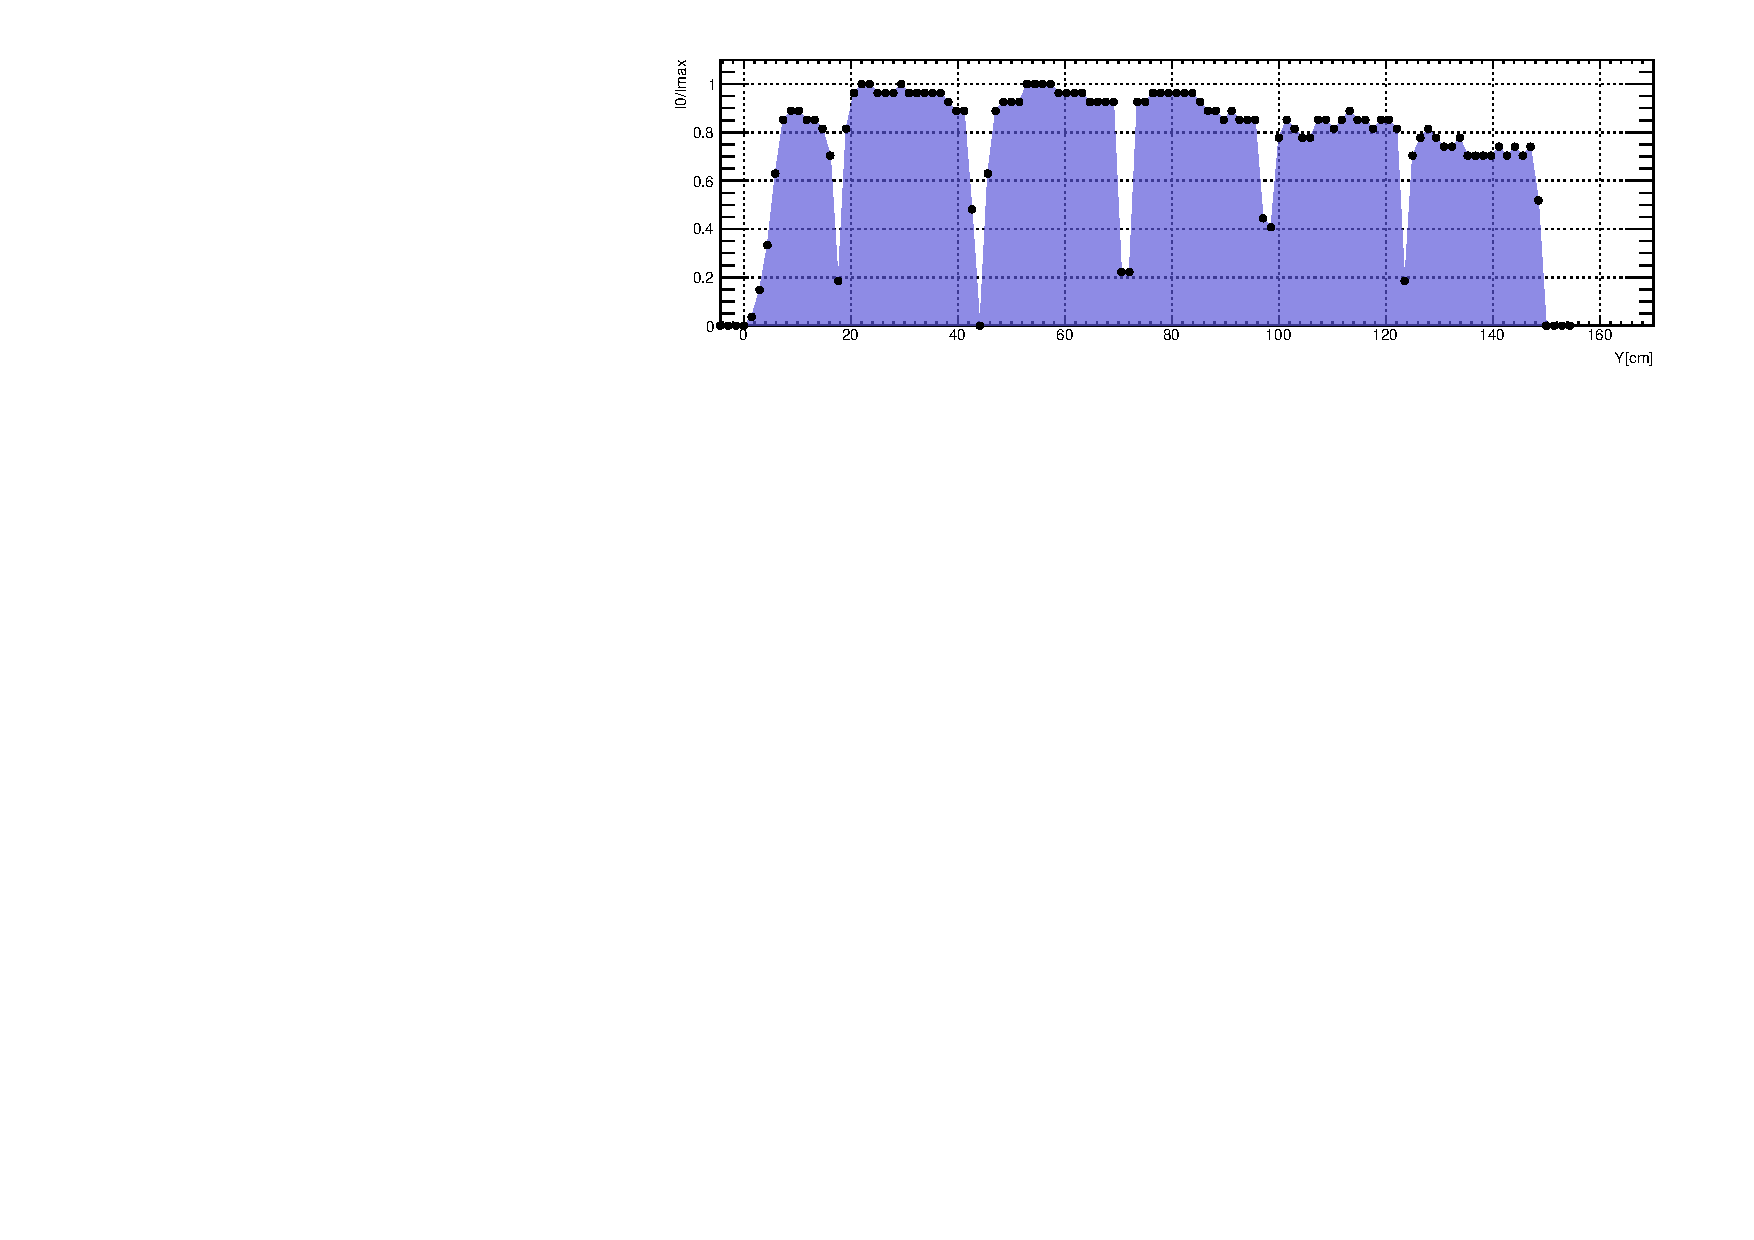
\includegraphics[width=0.9\textwidth]{relativecurrent.pdf}
		\hspace*{\fill}
		\captionsetup{margin=1cm}
	\caption{Moving across strips, wire-supports are present with minimum gain.}\label{fig:structure}
\end{figure}

At first glance, it is possible to observed the internal structure of the chamber with this test. Looking at the Figure
\ref{fig:structure} the current decreases when the gun is irradiating the places where the wire-supports are found. In
theses places a small gas volume is present, therefore less electrons can drift to the wires, resulting in less current
draw from the power supply.\par

If a better meshing of the irradiation places could be performed, identification of the wire-supports and the chamber
separation (small and large sector) could be obtained with good resolution. For internal parts of 20mm, a width from
\SIrange{17}{23}{mm} has been obtained with this test.\par

Interpolating the points (x, y, I), an overall picture can be obtained (Figure \ref{fig:xyscan}). The figure shows a line
with high current resulting from a missing wire on the Chamber3. More charge is collected by the neighbors when a wire
is missing, resulting from a longer drift path.\par

\begin{figure}[ht]
		\centering
		\hspace*{\fill}
		\begin{subfigure}[b]{0.45\textwidth}
			\centering
			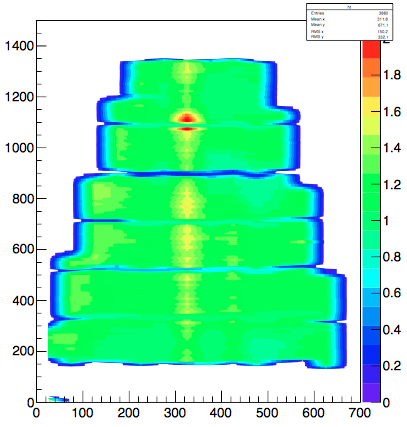
\includegraphics[width=\textwidth]{xy_scan.png}
			\caption{xy-scan Chamber3 sTGC Module \#0: missing wire}\label{fig:xyscan}
		\end{subfigure}
		\hfill
		\begin{subfigure}[b]{0.45\textwidth}
			\centering
			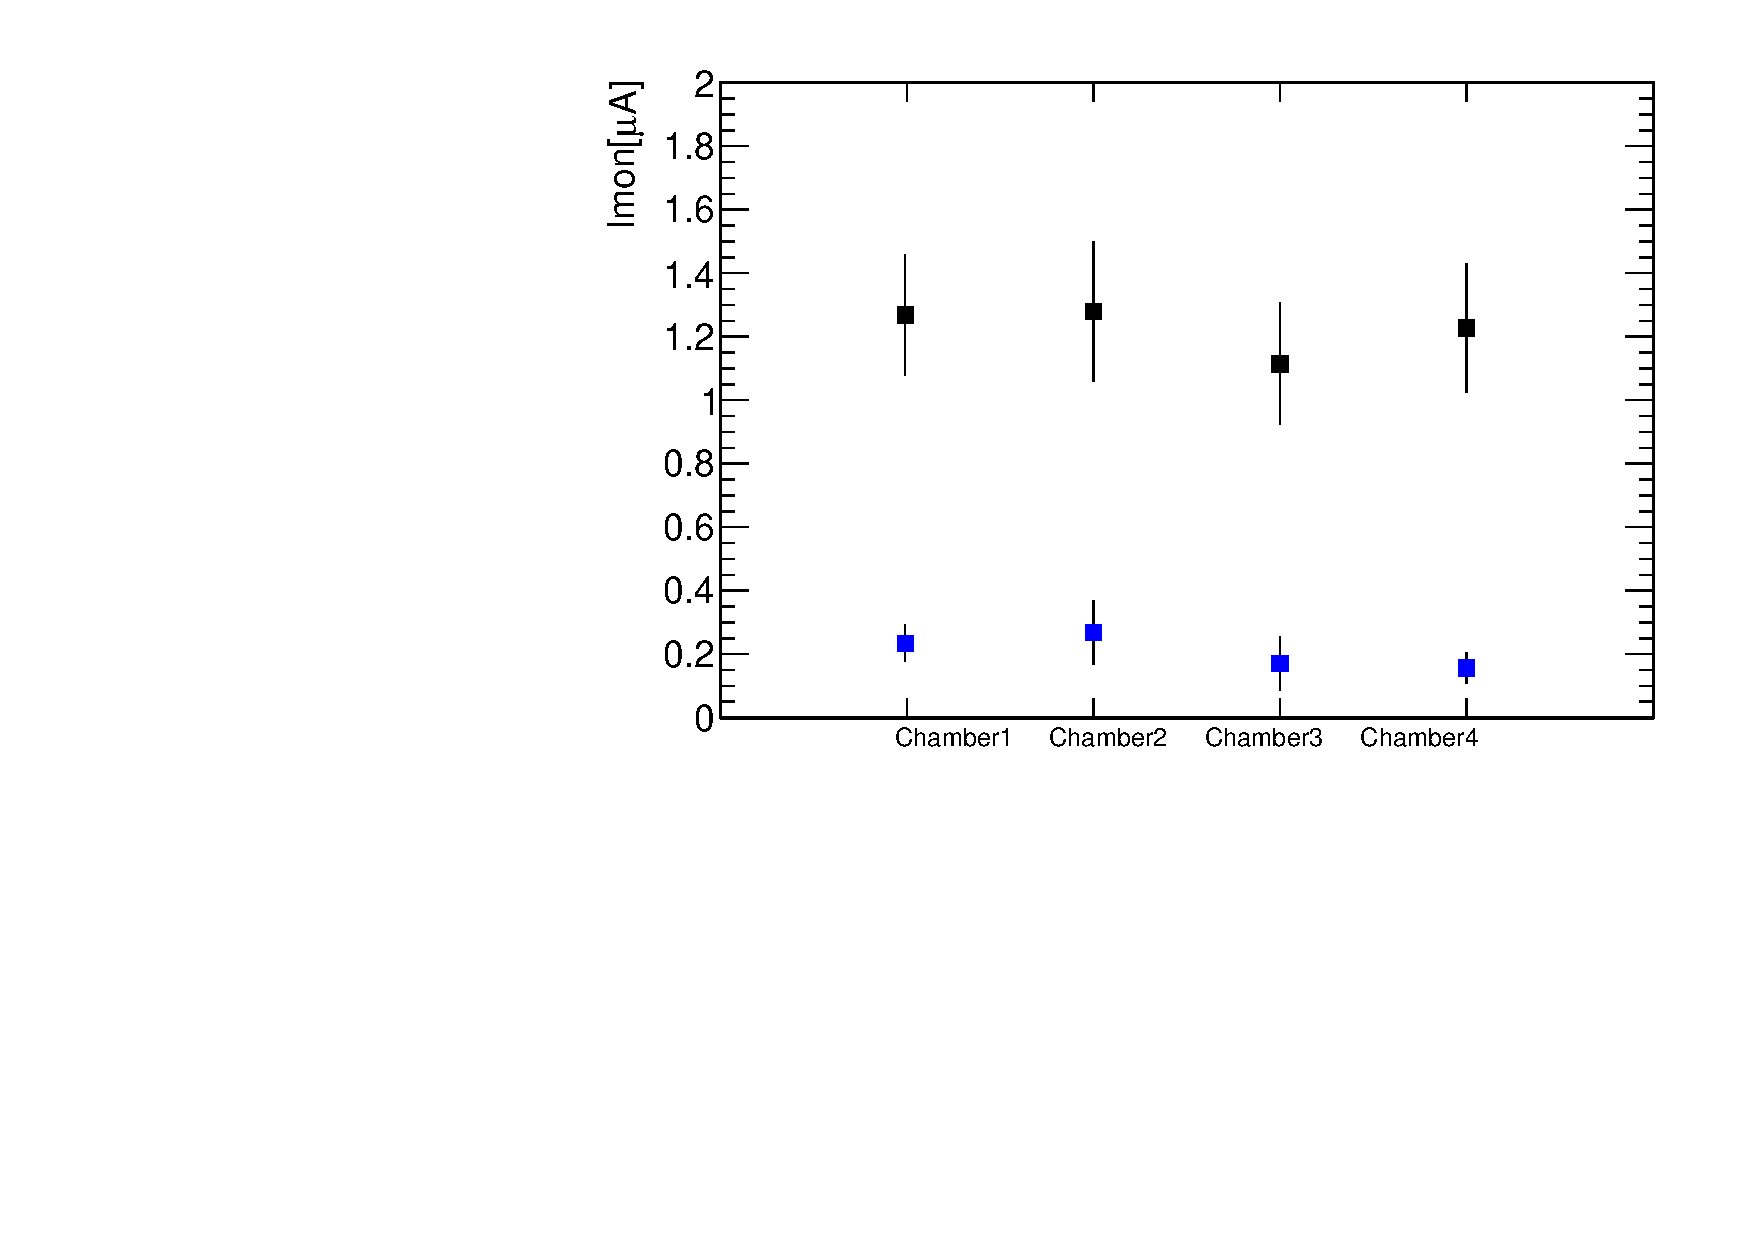
\includegraphics[width=\textwidth]{graphgain.pdf}
			\caption{Current draw at 2.5kV (blue) and 2.9kV(black)}\label{fig:draw}
		\end{subfigure}
		\hspace*{\fill}
		\caption{ }\label{}
\end{figure}


The graph on Figure \ref{fig:draw} shows the average current from each Chamber at two different working potential. The
average is calculated only for the sensitive area, hence, only values where the wire-support are not present
form part of the average. The average current values at 2.5kV and 2.9kV are \SI{200}{nA} and \SI{1.2}{\micro A} respectively.\par 

%Considering the approximate flux \cite{xgun}, $\Phi_{Xray} =$ $10^6$ [phonts/s mm$^2$] at \SI{30}{cm} is possible
%to estimate the flux at 5cm with a current tube 45 times higher. 
%\begin{equation}
%\mathrm{\Phi_0 = 45 \cdot 25 \cdot \Phi_{Xray}(r=30cm)\sim 10^9 \left[ photons/s\cdot mm^2\right ]}
%\end{equation}


\begin{table}
	\centering
	\begin{tabular}{ccccc}
	\hline
	& Chamber 1&Chamber 2 & Chamber 3 & Chamber4\\
	$\sigma$/mean\% 	
	 & 15.08\%  
& 17.18\%  
	 & 17.25\%  
	& 16.64\%  \\
	\hline\\
	\end{tabular}
	\caption{Uniformity gain}\label{table}
\end{table}

The Table \ref{table} summarizes the uniformity obtained, calculated as the RMS over the mean from the current draw
distribution for each chamber. The four chambers have less than 20\% of gain variation, which was expected from the
construction manual.\par



\section{Stability under high rate}\label{gifff}

One of the key feature of this detector is that it must be able to work under high particles flow
rates (\unit{15}{kHz/cm$^2$}), and the first step is
to check whether the device or its electronic components can handle this high rate.\par
\begin{figure}[ht]
	\hspace*{\fill}
	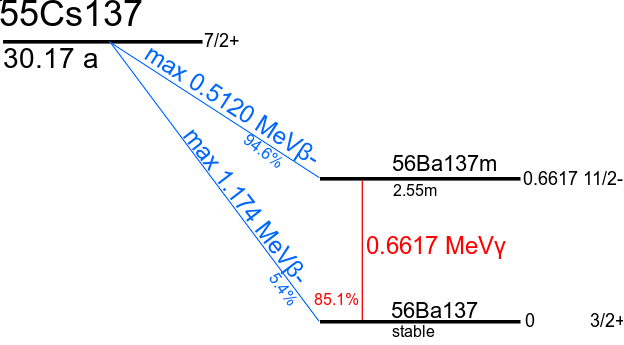
\includegraphics[width=0.4\textwidth]{cesiumdecay.png}
	\hspace*{\fill}
	\caption{Cesium-137 Decay scheme.}\label{cesium}
\end{figure}


For this purpose, the Module\#0 was
placed inside a new High Radiation Facility at CERN called GIF++\cite{gif}.
The installation has a Cesium-137 (Figure \ref{cesium}) as a gamma source with an activity of approximately
\unit{14.9}{TBq} (\unit{13.3}{TBq} during the test, August 2016). 
A system of movable lead attenuators (Figure \ref{filters}) for large irradiation zone allows attenuation factors
between 1 and $5\times10^5$
in several steps.\par 

In order to get a reference of the particle rate, a direct measurement setup was implemented with a  small size
(\SI{16,2x12,4}{cm} as sensitive area) sTGC as a {\bf Monitor}. A LVDS (Low voltage differential signaling) logical
signal from wires was obtained from an Amplifier Shaper Discriminator (ASD) board\cite{asdchip} connected to this
Monitor.\par

\begin{figure}[H]
		\hspace*{\fill}
		\begin{subfigure}[b]{0.25\textwidth}
			\centering
			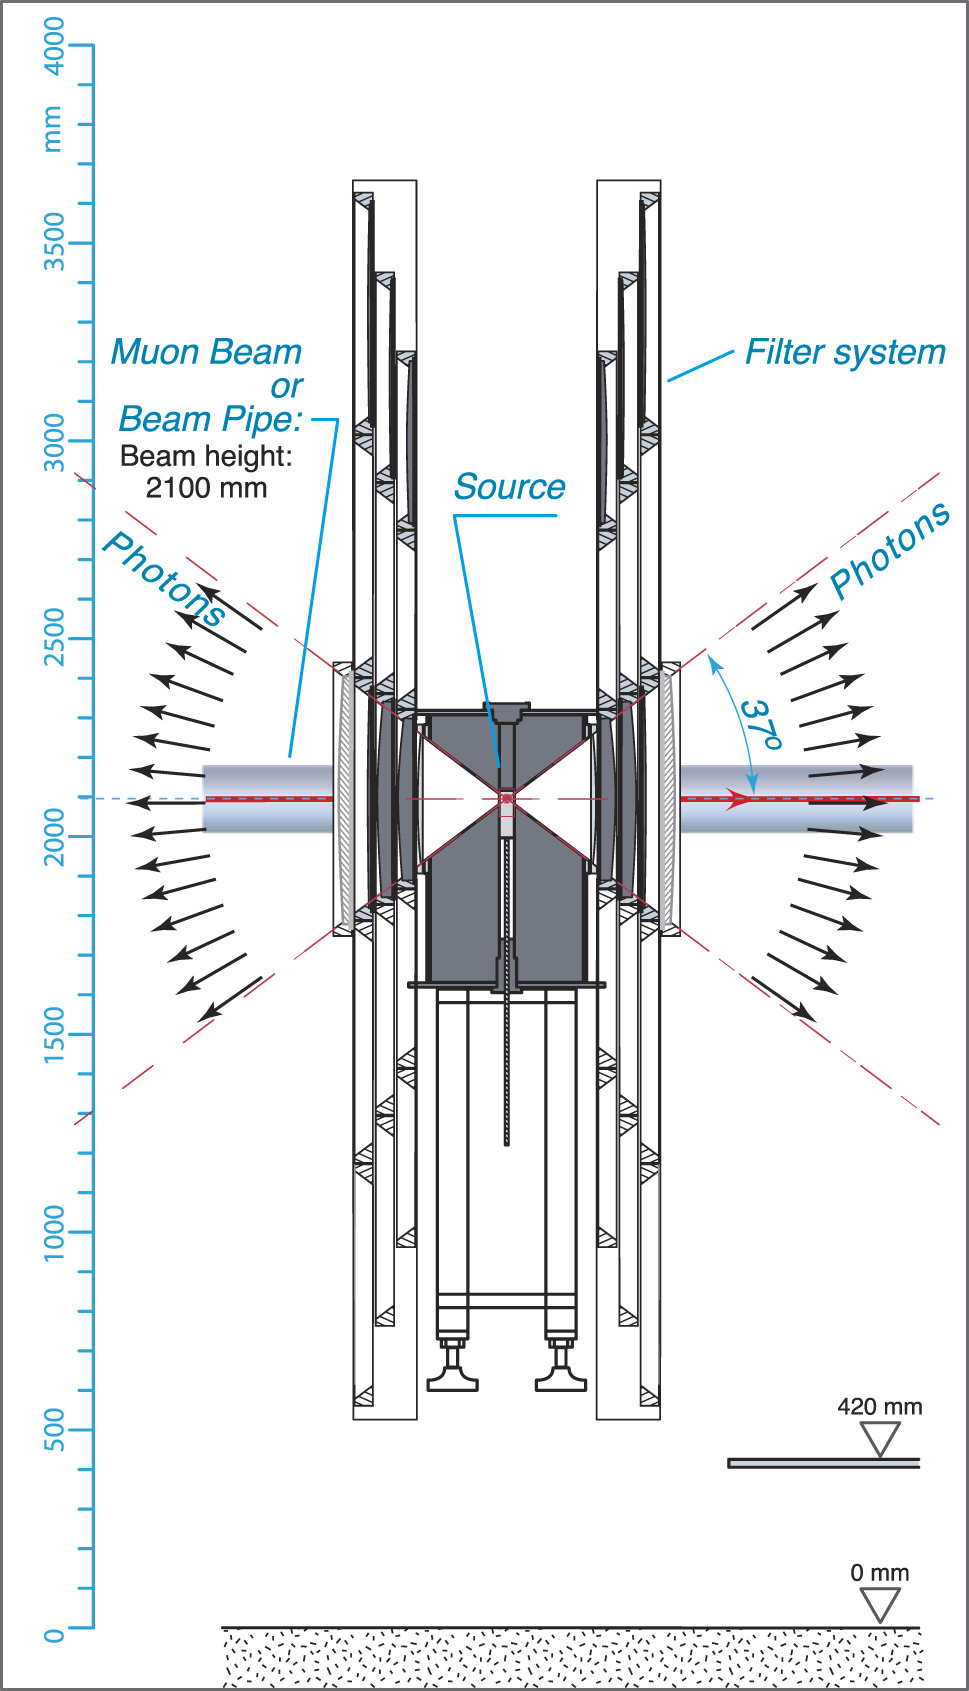
\includegraphics[width=\textwidth]{filters.png}
			\caption{Irradiator with filter system. }\label{filters}
		\end{subfigure}
		\hfill
		\begin{subfigure}[b]{0.45\textwidth}
			\centering
			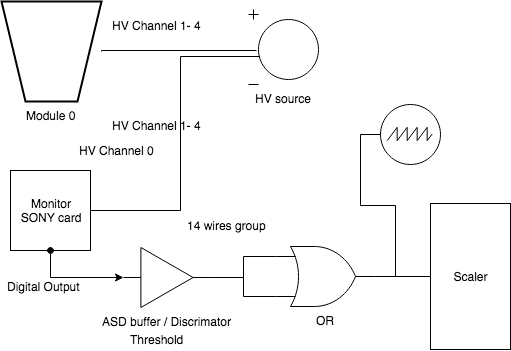
\includegraphics[width=\textwidth]{gif_setup.png}
			\caption{GIF++ setup.}\label{gifsetup}
		\end{subfigure}
		\hspace*{\fill}
		\captionsetup{margin=1cm}
		\caption{Three different rows with
		three lead (Pb) layers, each one with different thickness to provide multiples rates for the facility.}\label{}
\end{figure}

The ASD board provided the signal from 16 wires groups, all of them connected to a VME module (KEK ASD
buffer), which controls the threshold from the discriminator on the ASD and converts the LVDS to NIM signal. The 16
LVDS signals are converted into two NIM logical signals. The two outputs from the module are connected to a Scaler NIM
n145 which provides the number of positive NIM signals from the 16 channels in 10 seconds.\par

The Module\#0 and the Monitor were placed at 1.3m distance from the radioactive source. Both were connected in series
to the same gas line ($\mathrm{55 CO_2 : 45}$ n-pentane), and the temperature and pressure were recored to keep track of the working voltage. Most of the
time, the environmental conditions were measured at 25 Celsius degree and \unit{971}{mb}.\par 

The working potential for the chamber is 2850V at \unit{1}{b}. Since the gain is proportional to $E/P$, where $E$ is
the electrical field and $P$ the pressure inside the chamber, the voltages must be decreased by 2.9\% to compensate
the lower pressure, resulting in a 2765V as the new working point in this environment.\par 


To achieve the background rate for ATLAS (\unit{15}{kHz/cm$^2$}), the Monitor must register more than \SI{2680}{kHz} if
the sensitive area is considered. The sensitive area is calculated as the total area \SI{200}{cm^2} times the amount of
wires group connected to the ASD.\par

Four different attenuation factors were registered (10, 4.5, 2.2 and 1). On Figure \ref{fig:monrate} it is possible to
observe two sets of data with rates over than the expected one (red and blue). The other two sets of data emphasize the
{\it plateau} reached over \SI{2.7}{kV}. At the same time, the highest rate shows an inefficiency on voltages over
\SI{2.8}{kV} and the {\it plateau} is lost. Therefore, the data set with attenuation 2.2 (in red) is our reference.\par
\begin{figure}[H]
	\hspace*{\fill}
	\begin{subfigure}[b]{0.45\textwidth}
		\centering
		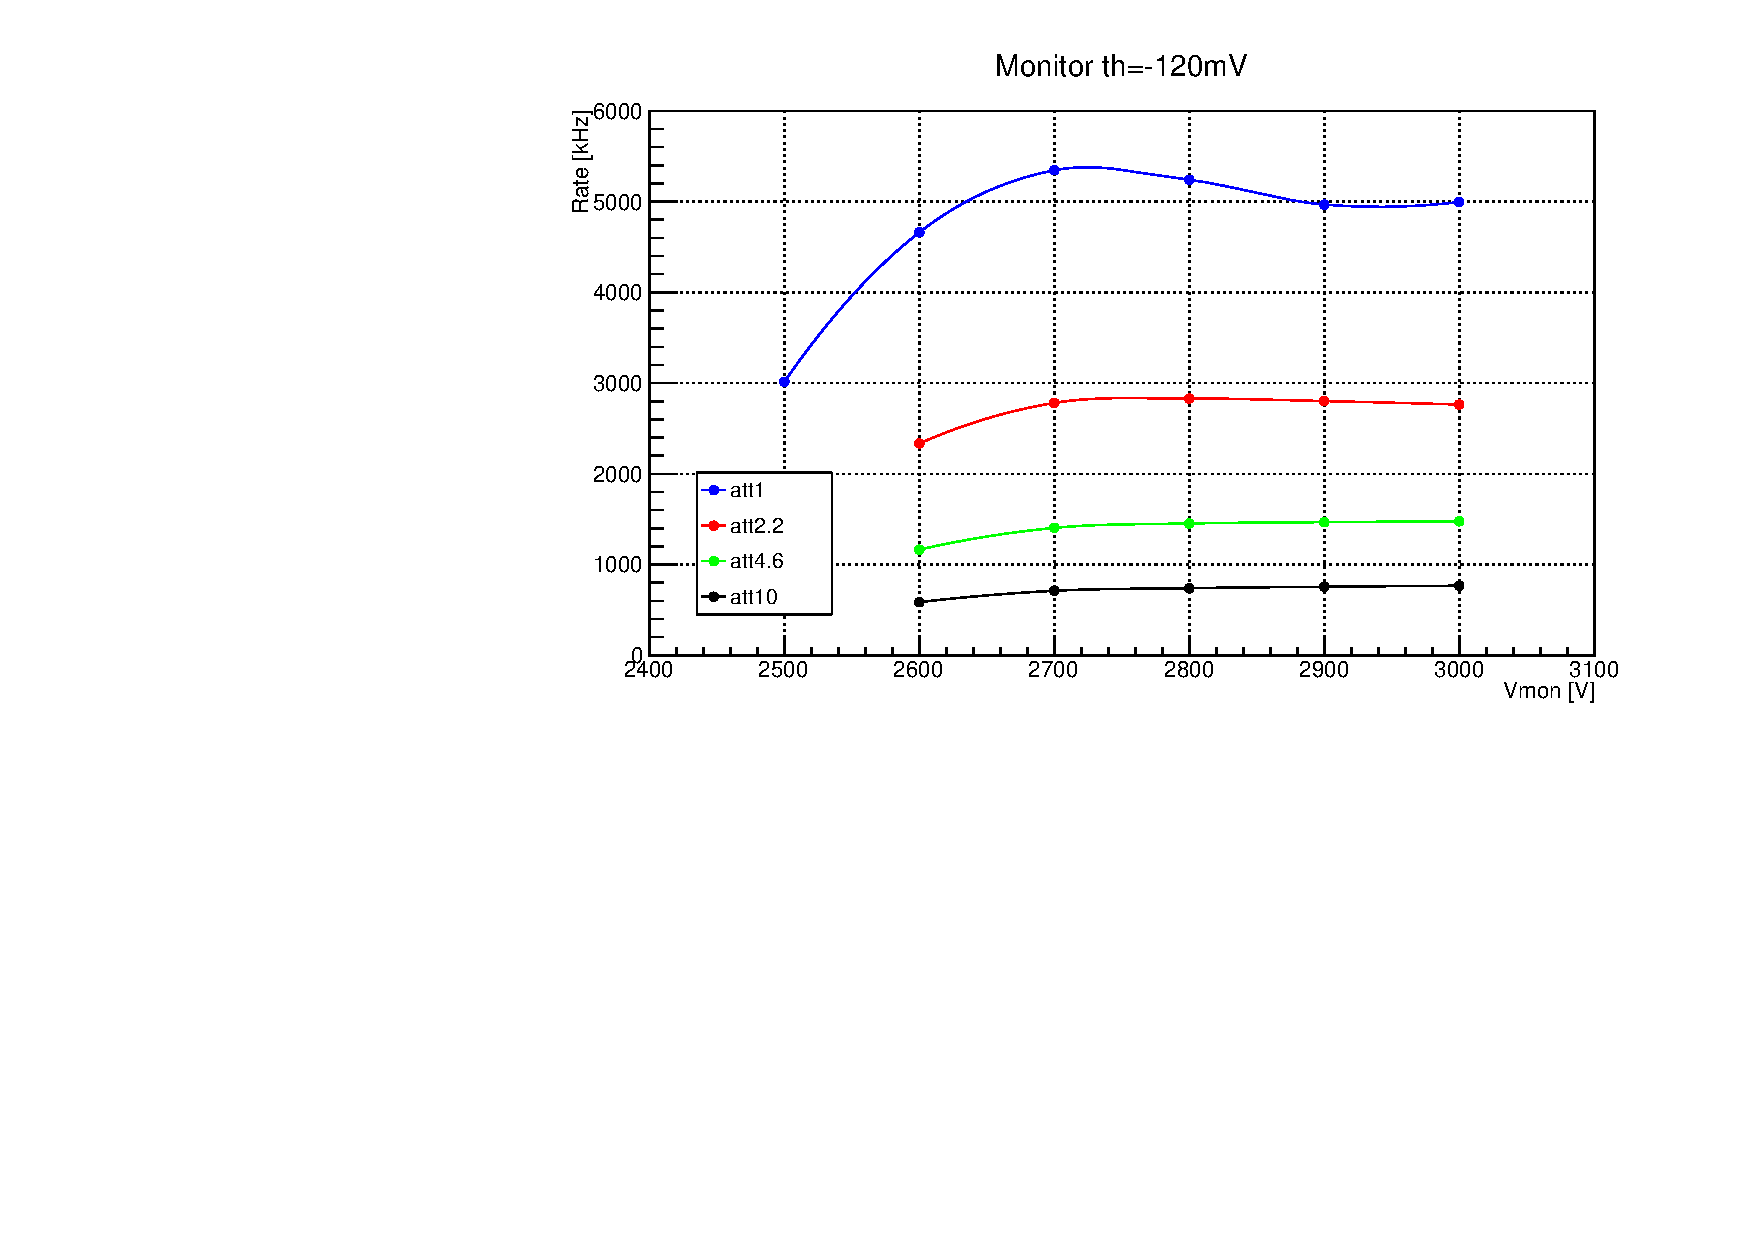
\includegraphics[width=\textwidth]{monitor.pdf}
		\caption{Different attenuation filters}\label{fig:monrate}
	\end{subfigure}
	\hfill
	\begin{subfigure}[b]{0.45\textwidth}
		\centering
		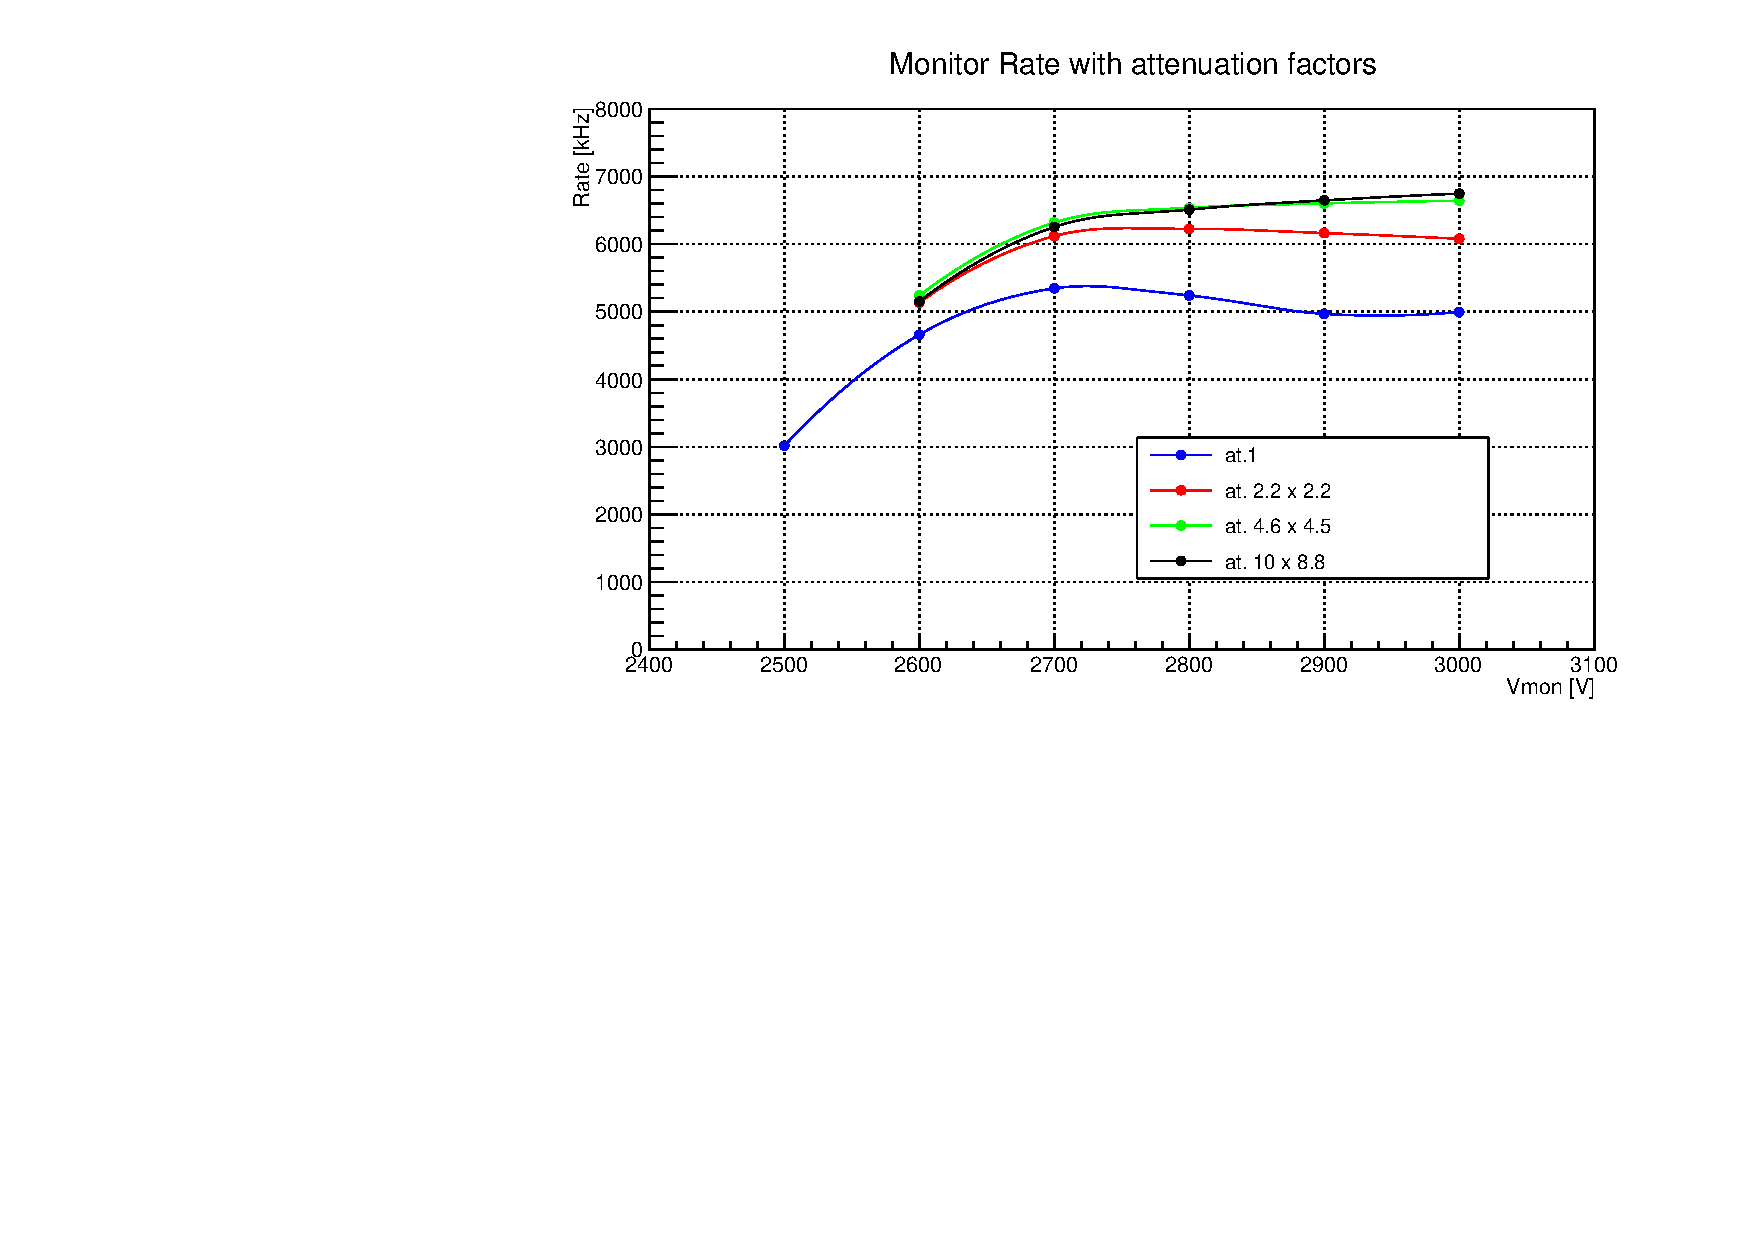
\includegraphics[width=\textwidth]{rate.pdf}
		\caption{Multiplying by att. Factors}\label{fig:filters}
	\end{subfigure}
	\hspace*{\fill}
	\caption{Rate on {\bf Monitor}}\label{}
\end{figure}

Multiplying the attenuation factors with each data set (Figure \ref{fig:filters}) should give us the expected rate with
no filters. However, the data set with factor 1 has \SI{5}{MHz} at working potential (2.9kV), while the expected rate
from data sets attenuation 10 and attenuation 4.6 is \SI{6.6}{MHz}. When comparing the rates from data set 1 with these,
we observe an efficiency of about 75\% of the  expected rate. Then, comparing the data set 2.2 with the lowest rates
results in approximately 93\% of efficiency.\par

These findings may suggest a change in the gamma spectrum emitted after the attenuation filters.  For a comprehensive
analysis, a detailed study of the spectrum can be found in Chapter \ref{spectrum}.\par


The flow rate recorded in data set 2.2 is \SI{28}{kHz/cm^2}, if we compensate the inefficiency the total flow rate is
\SI{30}{kHz/cm^2}, which is the double than expected as a background level for ATLAS. Therefore the sTGC detectors must
be tested against attenuation factor lower than 4.4.\par


\begin{figure}[t]
		\hspace*{\fill}
		\begin{subfigure}[b]{0.45\textwidth}
			\centering
			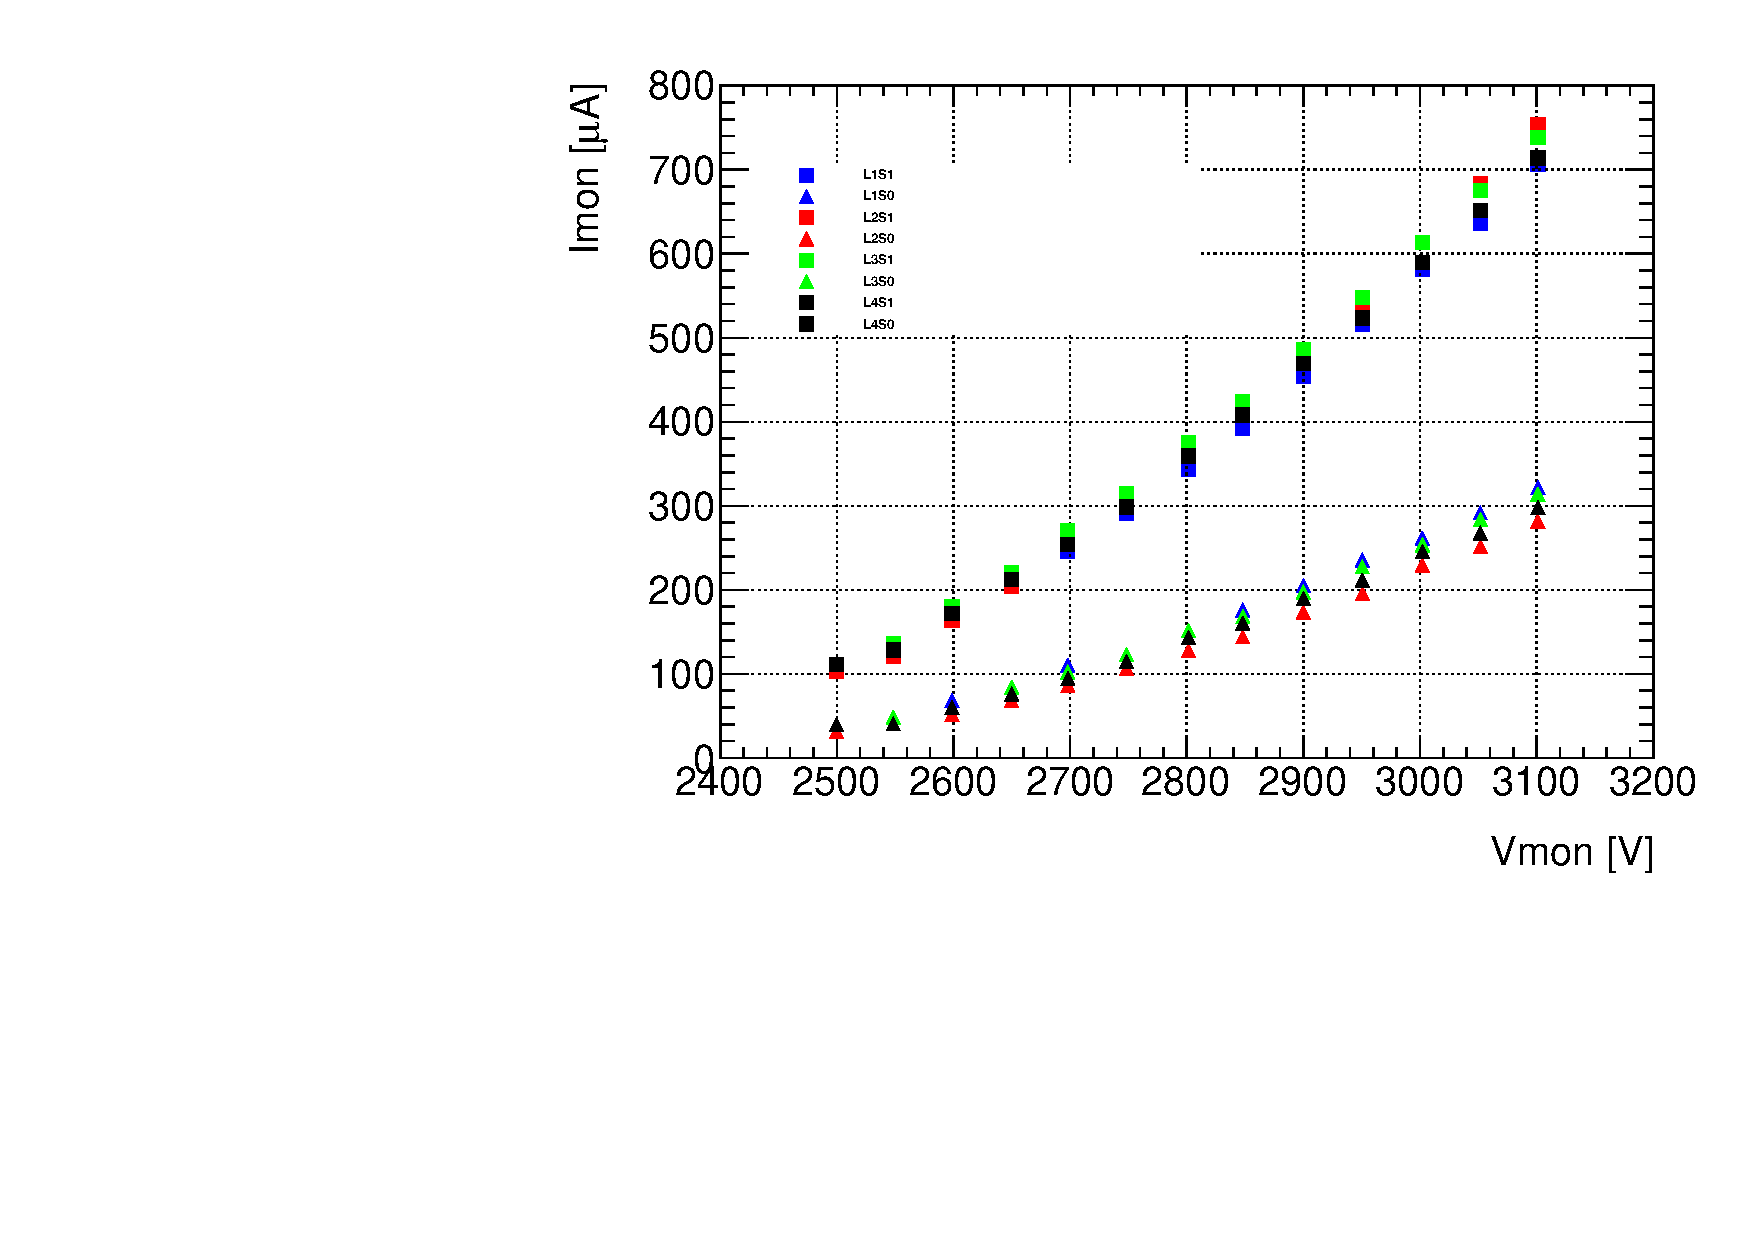
\includegraphics[width=\textwidth]{QS1_I_att1.pdf}
			\caption{Attenuation factor: 1}\label{fig:att1}
		\end{subfigure}
		\hfill
		\begin{subfigure}[b]{0.45\textwidth}
			\centering
			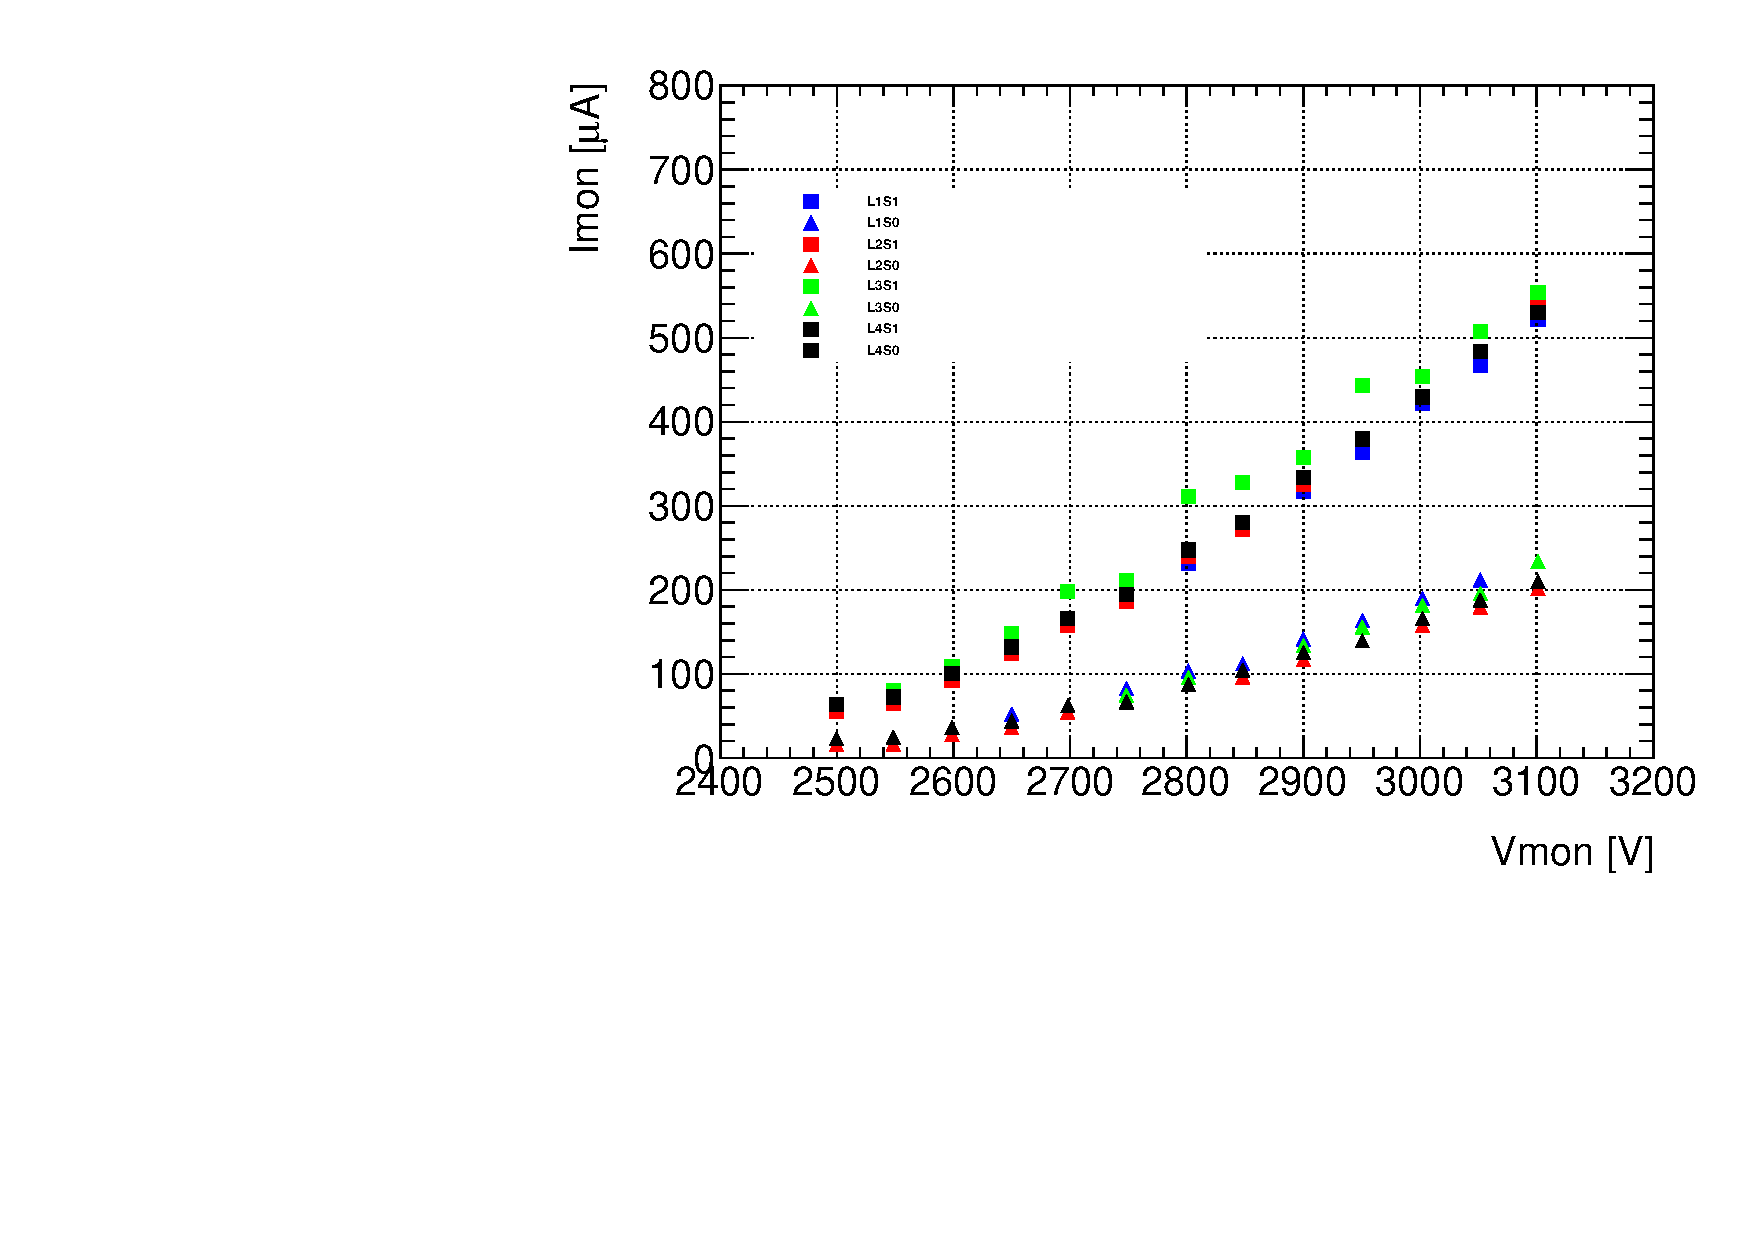
\includegraphics[width=\textwidth]{QS1_I_att22.pdf}
			\caption{Attenuation factor: 2.2}\label{fig:att22}
		\end{subfigure}
		\hspace*{\fill}\\
		\hspace*{\fill}
		\begin{subfigure}[b]{0.45\textwidth}
			\centering
			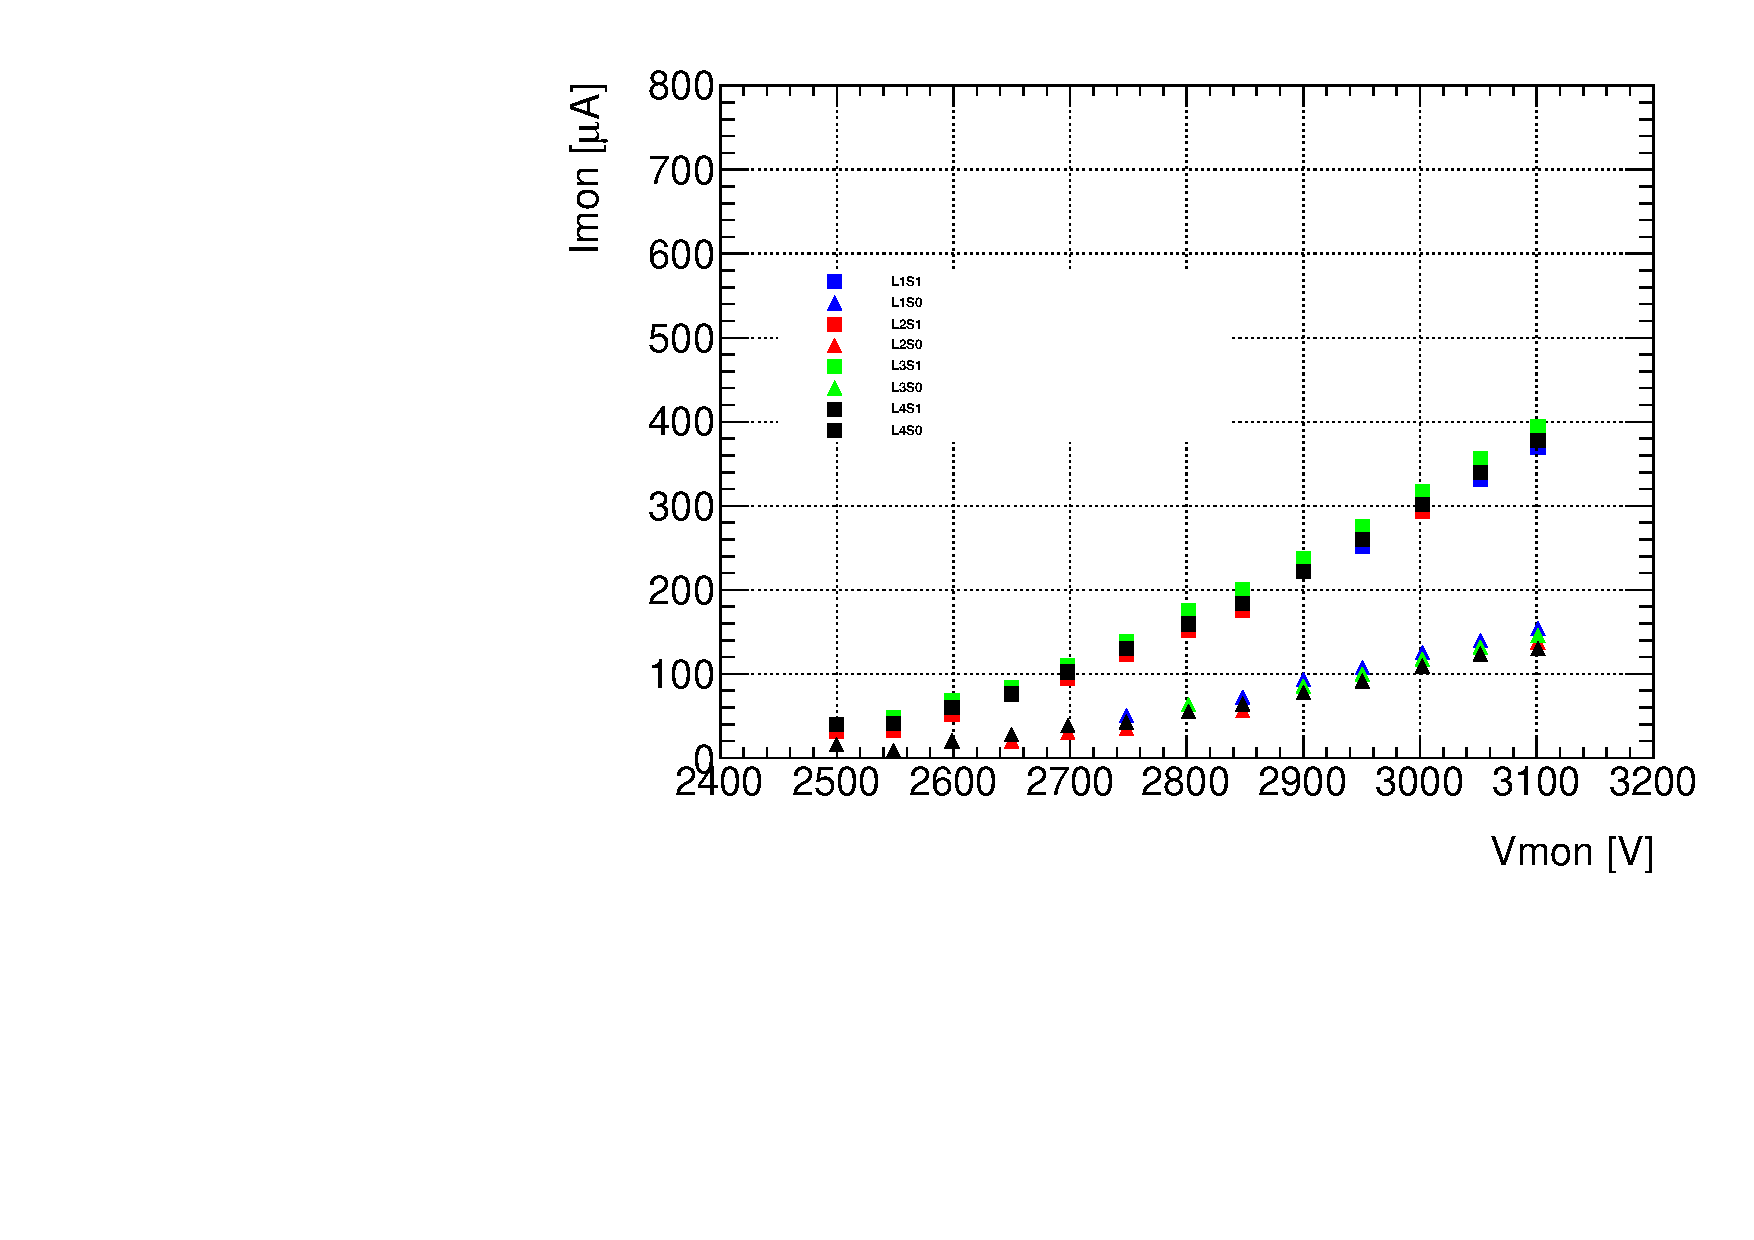
\includegraphics[width=\textwidth]{QS1_I_att46.pdf}
			\caption{Attenuation factor: 4.6}\label{fig:att46}
		\end{subfigure}
		\hfill
		\begin{subfigure}[b]{0.45\textwidth}
			\centering
			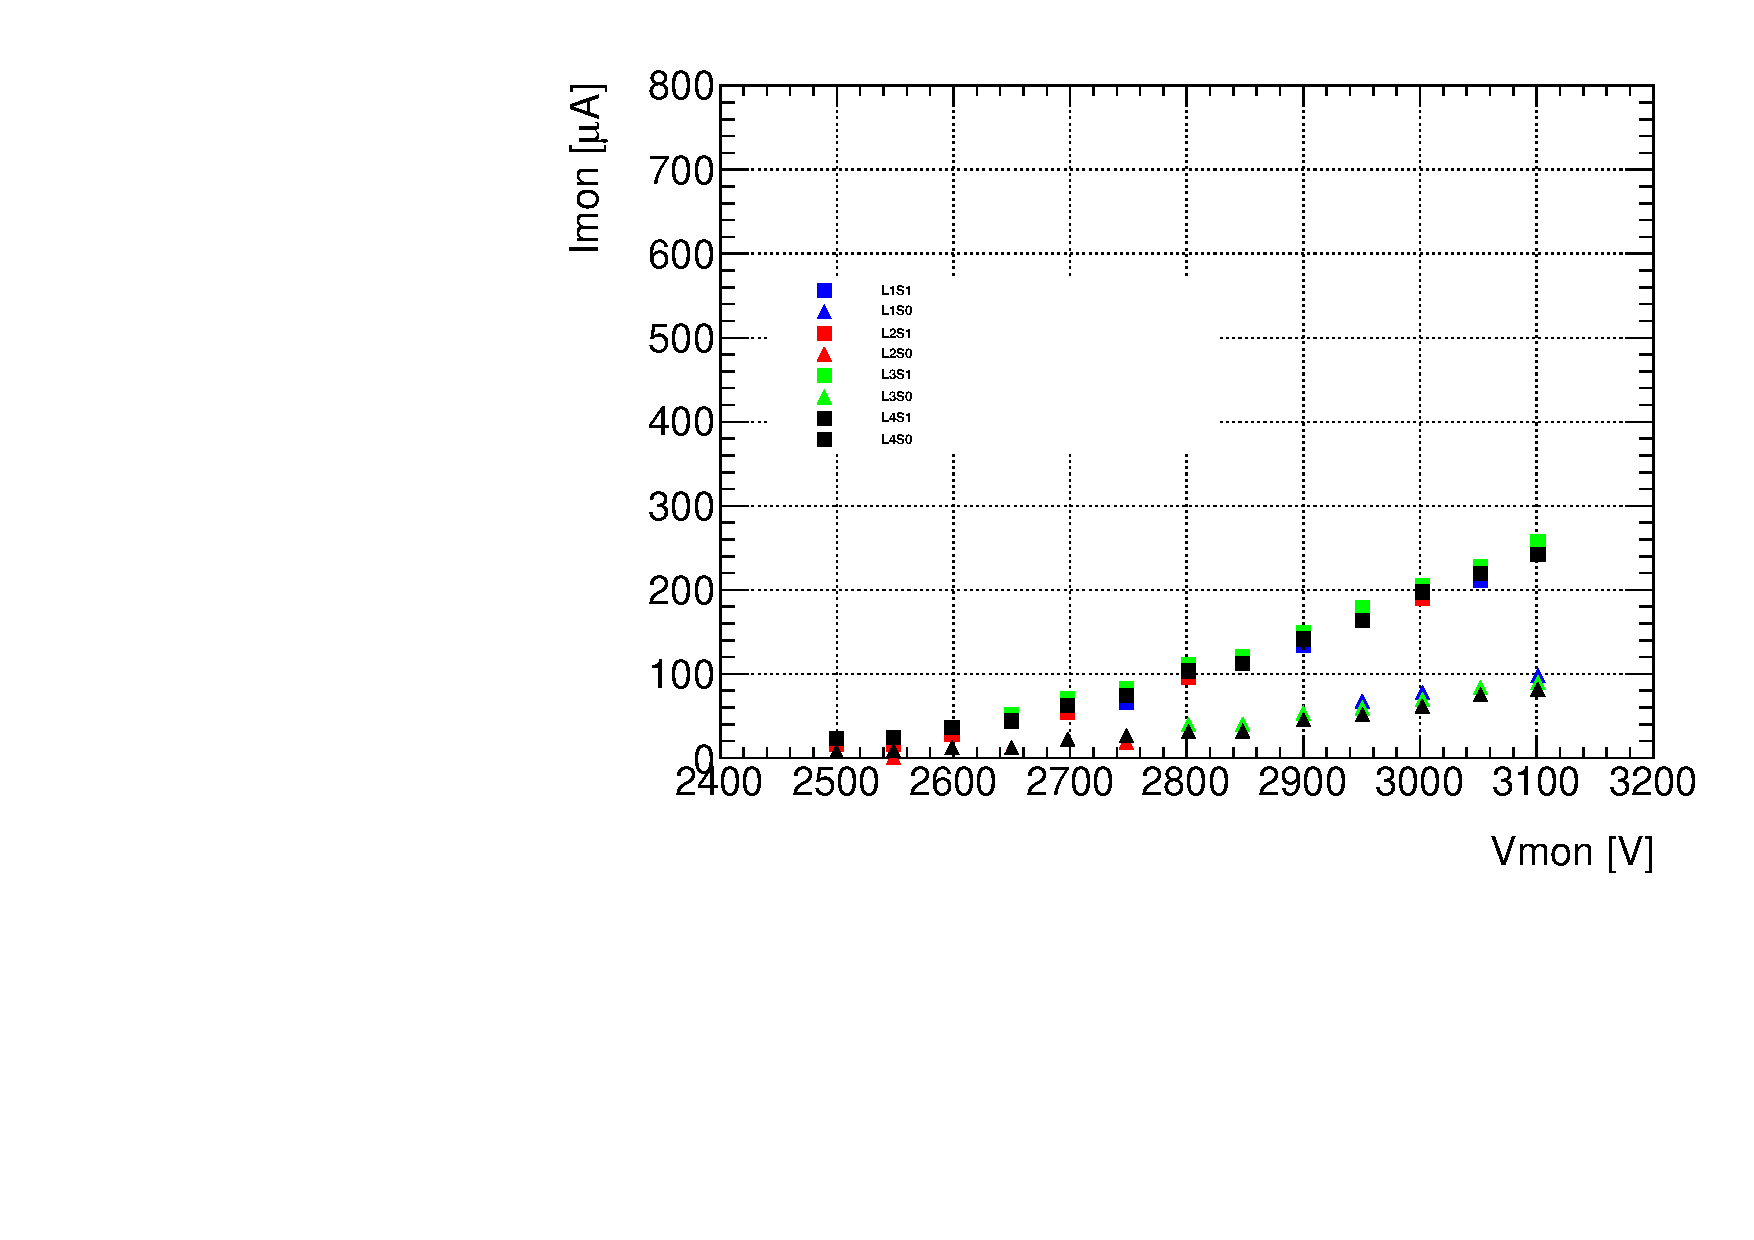
\includegraphics[width=\textwidth]{QS1_I_att10.pdf}
			\caption{Attenuation factor: 10}\label{fig:att10}
		\end{subfigure}
		\hspace*{\fill}
		\captionsetup{margin=1cm}
		\caption{Current registered on the power supply for each chamber, large (S1) and small sector (S0) against applied
		voltage on anode. }\label{gifresult}
\end{figure}

Once the Monitor is set, the quadruplet is connected to the high voltage power supply. Each layer is internally divided
in two sections, a small sector (S0) and large sector (S1). Each one of theses sector is powered independently on each
channel from the CAEN High Voltage power supply A1833P (\SI{4}{kV}/\SI{2}{mA} max). The current from each layer (two sectors
each one)	was recorded with a resolution of \SI{0.1}{\micro A}. Four different attenuation filters were applied, and the
results are shown in Figure \ref{gifresult}. 

\begin{equation}\label{eqn:delta}
	\Delta\%=\left|1-\frac{I_1/I_0}{A_1/A_0}\right|*100
\end{equation}


\begin{table}[ht]\footnotesize
	\centering
	\begin{tabular*}{0.7\textwidth}{rrcrcrcrc}
	 & \multicolumn{2}{c}{Layer 1} &\multicolumn{2}{c}{ Layer 2} &\multicolumn{2}{c}{ Layer 3
	}&\multicolumn{2}{c}{Layer 4}\\
	\hline
	$A_1$/$A_0$&\multicolumn{2}{c}{2.53}&\multicolumn{2}{c}{2.78}&\multicolumn{2}{c}{3.07}&\multicolumn{2}{c}{3.40}\\
	Filter & $I_1$/$I_0$ & $\Delta$\%& $I_1$/$I_0$ & $\Delta$\%& $I_1$/$I_0$ &$\Delta$\%& $I_1$/$I_0$ & $\Delta$\%\\ 	
	\hline
	10 	&2.49 &1.58  	&3.02 &8.63		&3.01 &1.95 	&3.08	&9.41 \\
	4.6 &2.34	&7.51 	&2.87 &3.24		&2.73 &11.07 	&2.87	&15.59\\
	2.2	&2.29 &9.49 	&2.79 &0.35		&2.68 &12.70 	&2.67	&21.47\\
	1		&2.22 &12.25 	&3.02 &8.63 	&2.45 &20.19 	&2.49	&26.76\\
	\hline
	\end{tabular*}
	\centering
	\captionsetup{margin=1cm}
	\caption{Comparison between sensitive area ratio ($A_1$/$A_0$) from large and small sectors with the ratio of current
	($I_1$/$I_0$) at 2.9kV. A percentage difference column ($\Delta \%$ defined in equation \ref{eqn:delta}) is calculated to
	highlight the incremental disagreement as the gamma rate and the area ratio increases.}\label{aratio}
\end{table}
\begin{figure}[hb]
		\hspace*{\fill}
		\begin{subfigure}[b]{0.45\textwidth}
			\centering
			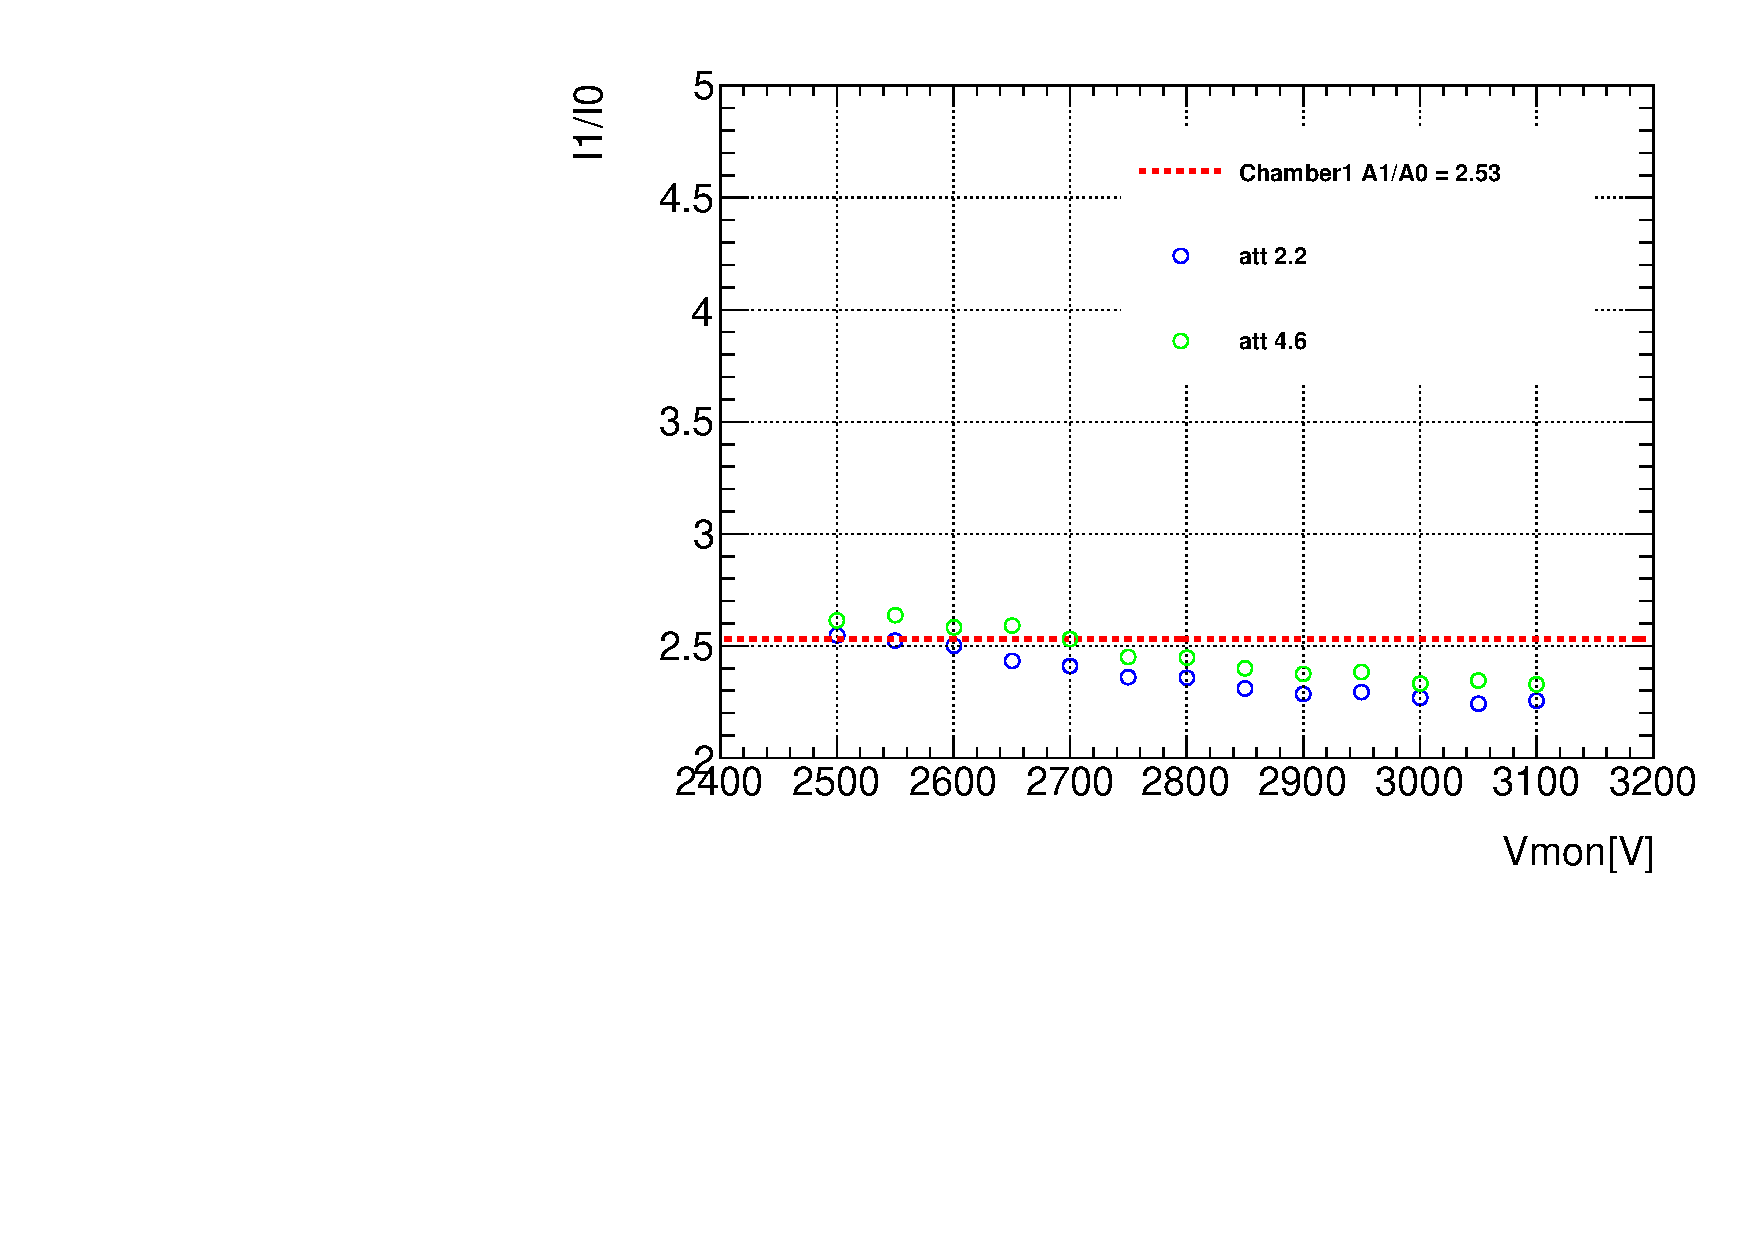
\includegraphics[width=\textwidth]{a1.pdf}
			\caption{Chamber 1, $A_1/A_0=$2.53}\label{fig:a1}
		\end{subfigure}
		\hfill
		\begin{subfigure}[b]{0.45\textwidth}
			\centering
			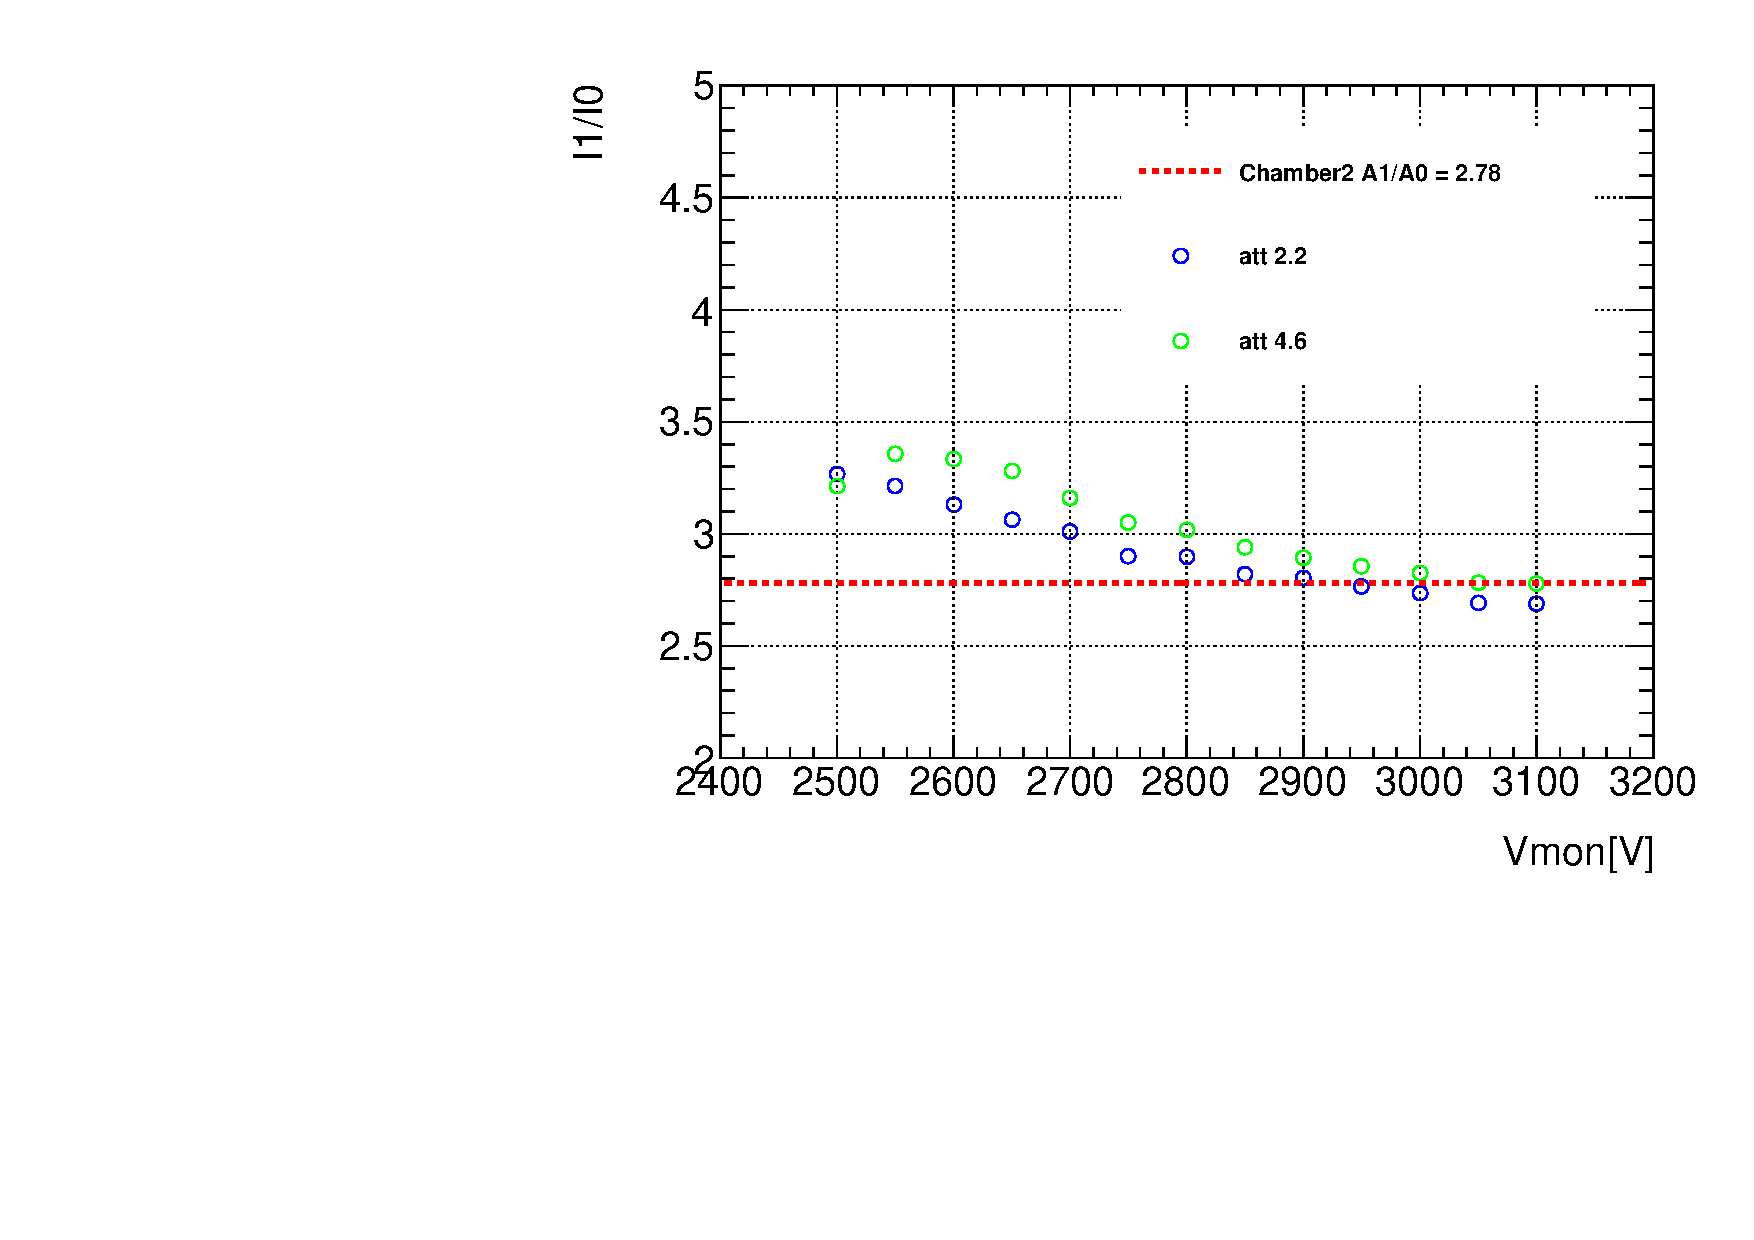
\includegraphics[width=\textwidth]{a2.pdf}
			\caption{Chamber 2, $A_1/A_0=$2.78}\label{fig:a2}
		\end{subfigure}
		\hspace*{\fill}\\
		\hspace*{\fill}
		\begin{subfigure}[b]{0.45\textwidth}
			\centering
			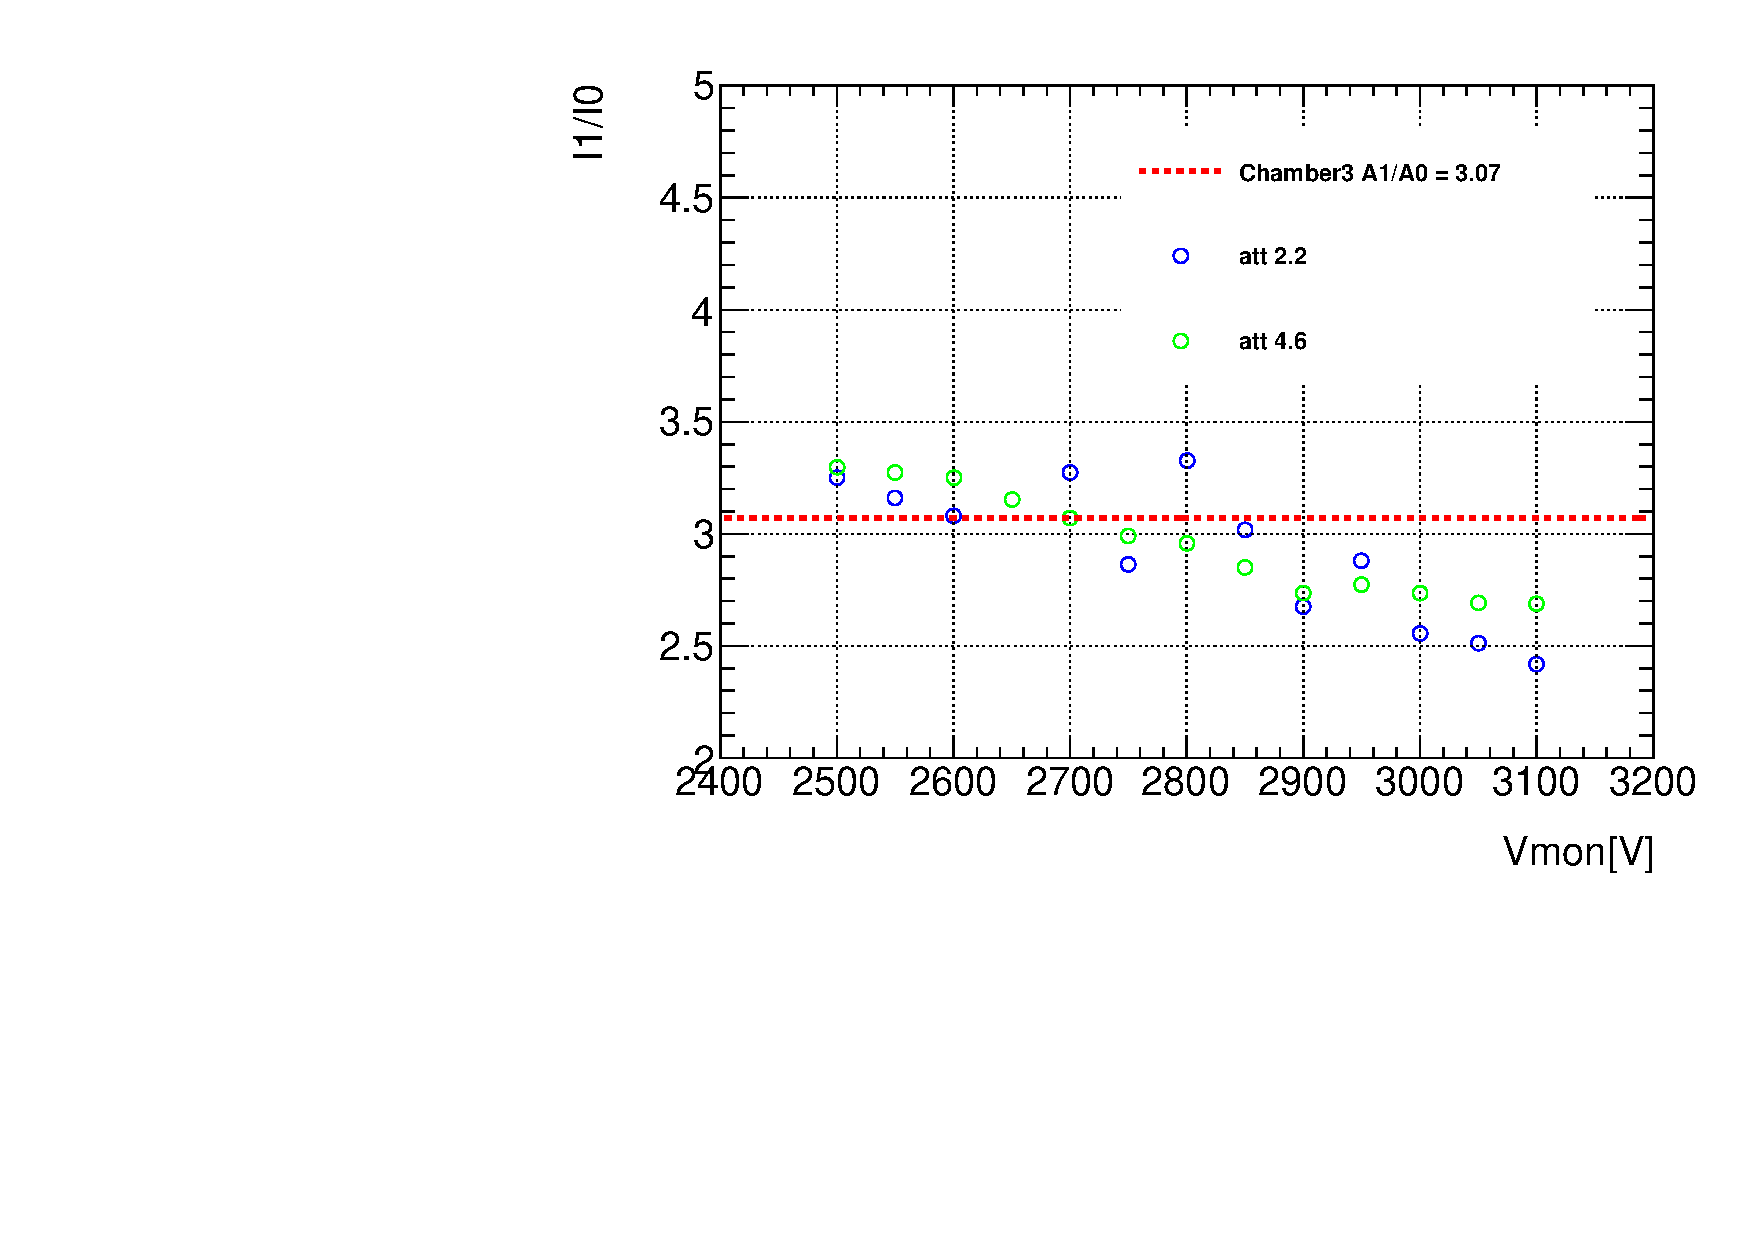
\includegraphics[width=\textwidth]{a3.pdf}
			\caption{Chamber 3, $A_1/A_0=$3.07}\label{fig:a3}
		\end{subfigure}
		\hfill
		\begin{subfigure}[b]{0.45\textwidth}
			\centering
			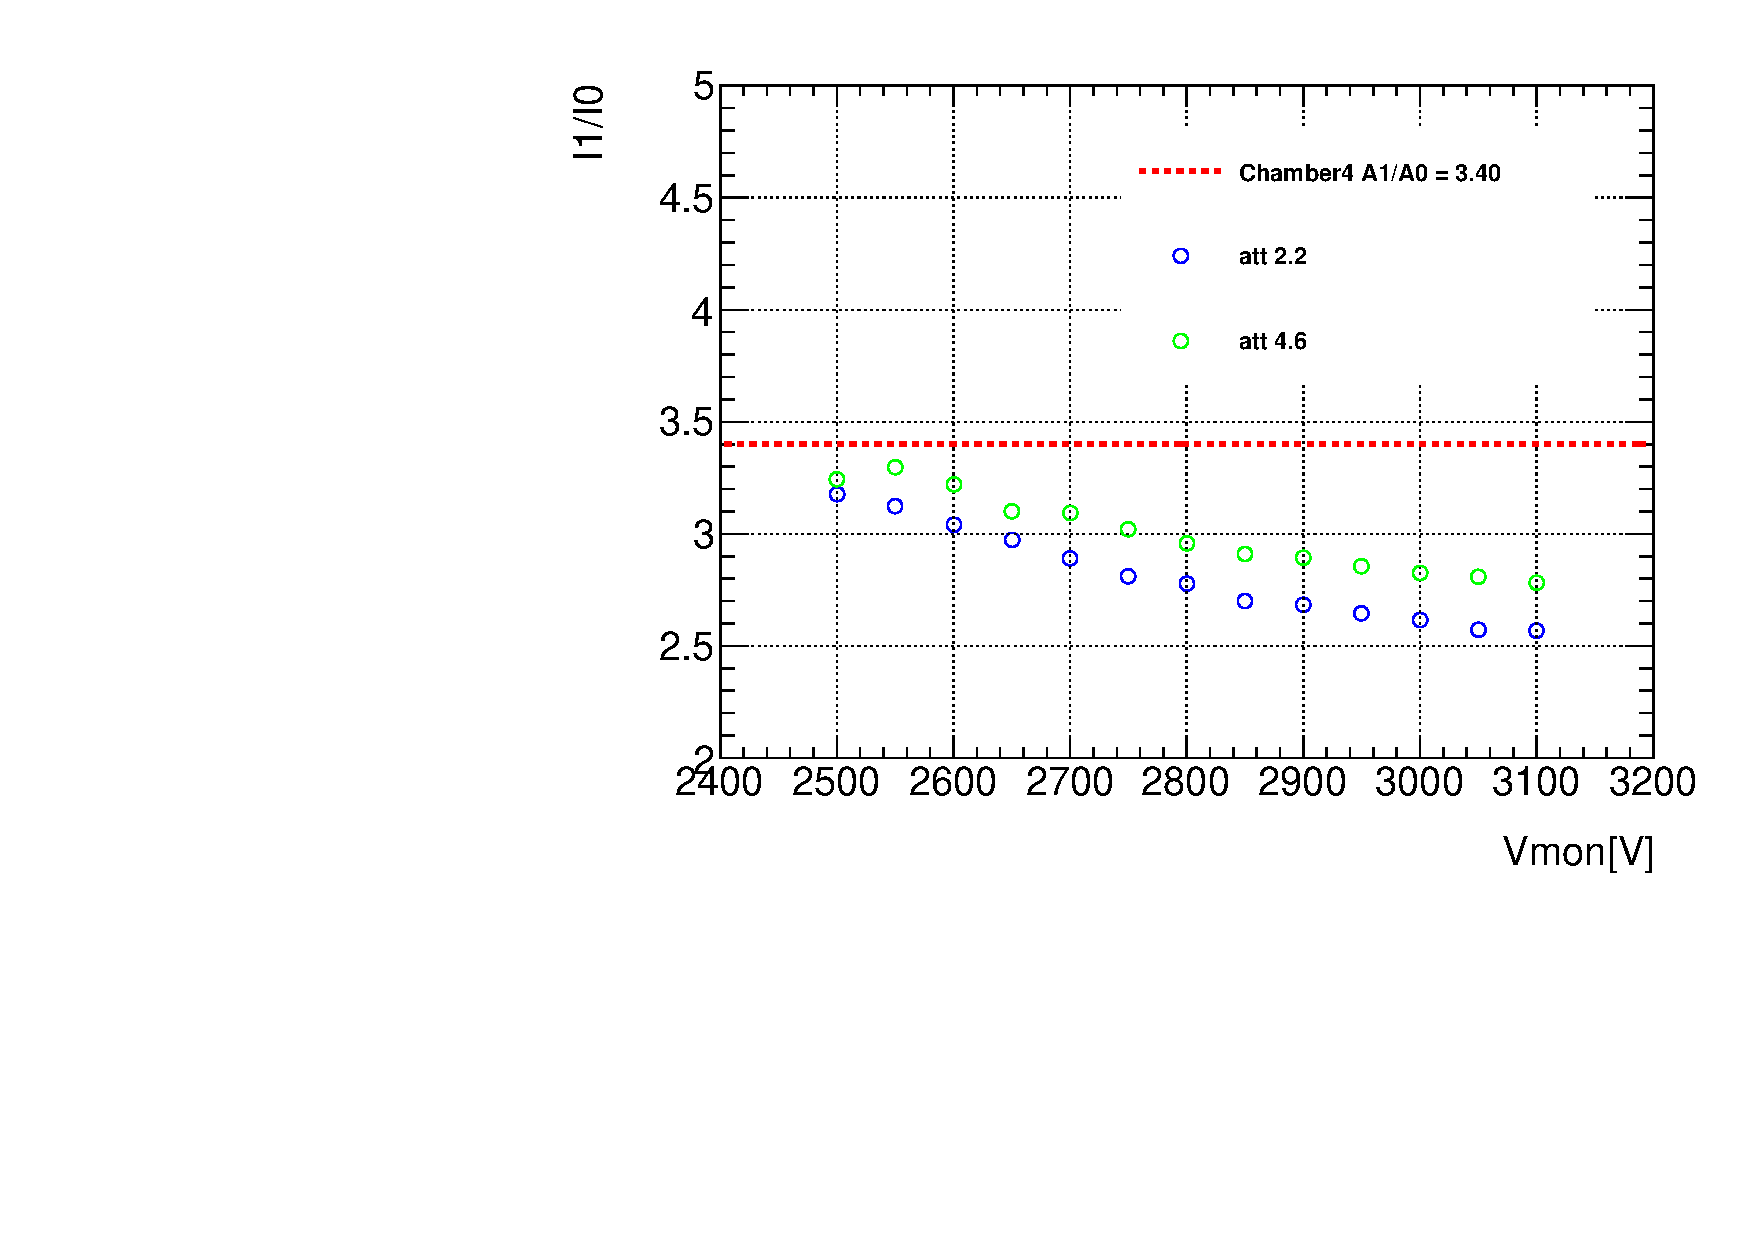
\includegraphics[width=\textwidth]{a4.pdf}
			\caption{Chamber 4, $A_1/A_0=$3.40}\label{fig:a4}
		\end{subfigure}
		\hspace*{\fill}
		\captionsetup{margin=1cm}
		\caption{Current ratio $I_1/I_0$ for two different rates compared with the area ratio $A_1/A_0$ at different anode
		voltage. The Chamber 3 in (c) has a missing wire in the large section ($A_1$), therefore the area ratio
		must be slightly lower and an increase of the current can be expected for the same reason.}\label{plotratios}
\end{figure}

These results shows a linear dependency of voltage, with lower resistance as the rate of particles is increased. It is
also important to notice that each wire group is connected to a \SI{10}{\mega\ohm} resistor, however not all the wires
have the same length (the chamber has a trapezoidal shape), resulting in a lower voltage drop from the external groups where the
wires are shorter (collecting less charge).\par

The Table \ref{aratio} compares the area ratio between the internal sections of each chamber with the current registered
for each set of measurements. The effect of dropping voltage appears to be the explanation of the incremental
disagreement of the area ratio as the rate increases.\par
The set of graphs shown in Figure \ref{plotratios} highlights the
disagreement between different working voltages for two different rates. 

These two sets of data are the expected rates for
the large and small sector on the sTGC QS1. Hence, it is important to compare these ratios with the amount of current
registered by both sectors. As the area ratio increases, the current ratio decreases, which suggests the use of different HV
resistors for the external wires groups to produce an homogeneous voltage drop. \par


	%----------------- SPATIAL RESOLUTION ---------------


\section{Spatial Resolution}\label{resolution}

In order to achieve the precision reconstruction of tracks (offline) with a spatial resolution of about
\unit{100}{\micro m} per sTGC layer, and fast trigger on the region of interest (ROI) with Pads, two test beams were
done.\par

In the spring of 2014, the Weizmann Institute of Science in Israel built the first full-size sTGC quadruplet detector of
dimensions \unit{1.2x1.0}{m$^2$}. This prototype consists of four sTGC strips and pad layers and is constructed using the
full specification of one of the quadruplets to be used in the NSW upgrade (the middle quadruplet of the small sector).
The first test beam experiment took place at Fermilab with one goal in mind, to determine the position resolution of a
full-size sTGC.\par

\begin{figure}[t]
\centering
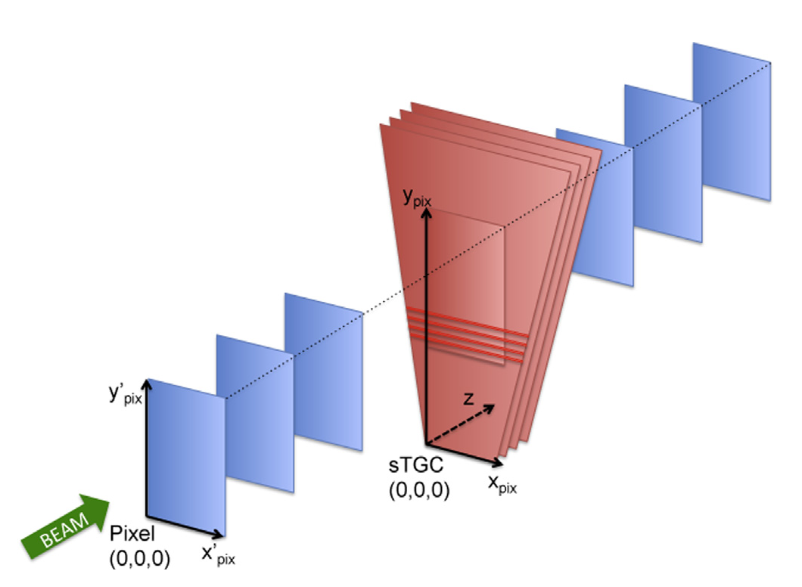
\includegraphics[width=0.5\textwidth]{telescope.png}
\caption{\small Schematic diagram of
the experimental setup at Fermilab and coordinate systems used. Three layers of silicon pixel sensors are positioned
before and after the sTGC detector.The dimensions are not to scale.}\label{fig:telescope}
\end{figure}


EUDET pixel telescope was used as a reference to measure the beam position, using the technology of 6 Minimum Ionizing
MOS Active Pixel Sensor (Mimosa26) detectors with $\approx 5 \mu$m position resolution. Three telescopes are placed in
front of the beam, and three after the sTGC as is shown in Figure \ref{fig:telescope} with \unit{15}{cm} between them
and \unit{64}{cm} between each arm.  Each Mimosa26 detector has an active area of \unit{2.24}{cm$^2$} made of CMOS
pixel matrix of 576 rows and 1152 columns with \unit{18.4}{\micro m} pitch.\par


A \unit{32}{GeV} pion beam was used at the rate of \unit{1}{kHz} over a spot of \unit{1}{cm$^2$} giving to the sTGC a
very precise pion trajectory thanks to the EUDET telescope.  Event triggering was controlled by a custom Trigger Logic
Unit (TLU). The TLU received signals from two \unit{1x2}{cm$^2$} scintillators placed in front and behind the telescope.
The TLU generated the trigger signal that was distributed to the telescope and the sTGC readout electronics, which
consists of a first application-specific integrated circuit (ASIC) called VMM1 which has the ability to read out both
positive (strips, pads) and negative (wires) polarity signals, on 64 individual readout channels.\par
	
The VMM1 analog circuit features a charge amplifier stage followed by a shaper circuit and outputs the analog peak value
(P) of the signal.\par
	
The readout of the ASIC is zero suppressed and thus only peak values of channels with signals above a predefined
threshold are read.  At the same time, the VMM1 may be programmed to provide the input signal amplitude of channels
adjacent to a channel above threshold (neighbor-enable logic).\par
	
The precise position of a charged particle traversing an sTGC gas volume can be estimated from a Gaussian fit to the
measured charge on adjacent readout strips (referred to as strip-clusters from here on). Given the strip pitch of
\unit{3.2}{mm} and sTGC geometry, charges are typically induced on up to five adjacent strips. \par

The spatial sampling of the total ionization signal over a small number of readout channels means that a precise
knowledge of each individual readout channel baseline is necessary in order to achieve the best possible measured
spatial resolution. \par

The baseline of each individual readout channel was measured by making use of the neighbor-enabled logic of the VMM1 and
its internal calibration system. \par

Test pulses were sent on one readout channel with the neighbor-enabled logic on, and baseline values were obtained by
reading out the analog peak values of the two channels adjacent to the one receiving a test pulse.\par
	
The silicon pixel hit positions were then used for reconstructing straight three dimensional charged-particle tracks.  A
track quality parameter was obtained for each fitted pion track based on the $\chi^2$ of the track-fit. A small value of
the track quality parameter corresponds to a straight track and a cut on this parameter can therefore be used to
mitigate multiple scattering which are not considered in this analysis.\par


\subsection{Analysis Model}


\subsubsection{Pixel telescope analysis}


In this model the intrinsic position resolution is obtained comparing the extrapolated beam trajectory from the pixel
detectors with the measurements in each of the sTGC quad planes. Each layer is analyzed separately to reduce the effect
of the multiple scattering and only tracks with $\chi^2<10$ are considered for the same reason. From Figure
\ref{fig:telescope} one can see that the {\it y-axis} is defined perpendicular to the strips, therefore sTGC
strip-clusters provide measurements of the particle position in the y-direction($y_{\mathrm{sTGC}}$).\\

The position resolution is directly related to the profile of induced charge on the strips. The particle position is
estimated from a Gaussian fit to the induced charge distribution on the strips. The neighbor-enabled logic of the VMM1
was used. Strip-clusters with induced charge in either 3, 4 or 5 adjacent strips are selected.\par
	
The pixel telescope tracks provide both coordinates, $x_{\mathrm{pix}}$ and $y_{\mathrm{pix}}$ at the position of the
sTGC layer studied. The spatial resolution measurement is obtained by fitting the residual distribution
$y_{\mathrm{sTGC}}$  and $y_{\mathrm{pix}}$ with a Gaussian model.\par


\begin{figure}[ht]
	\centering
	\hspace*{\fill}
	\begin{subfigure}[b]{0.45\textwidth}
		\centering
		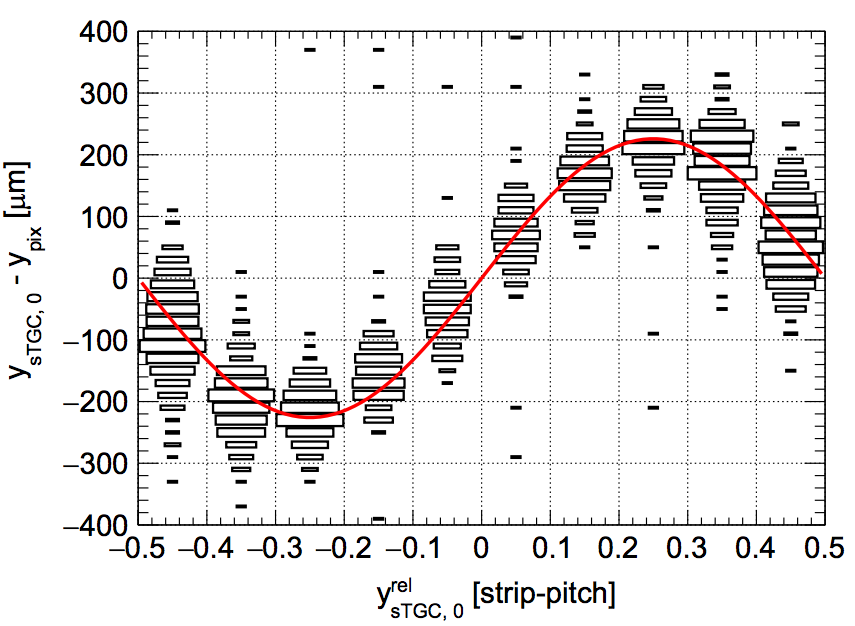
\includegraphics[width=\textwidth]{strip-pitch.png}
		\caption{The differential non-linearity for sTGC strip-clusters}\label{fig:pitchfit}
	\end{subfigure}
	\hfill
	\begin{subfigure}[b]{0.45\textwidth}
		\centering
		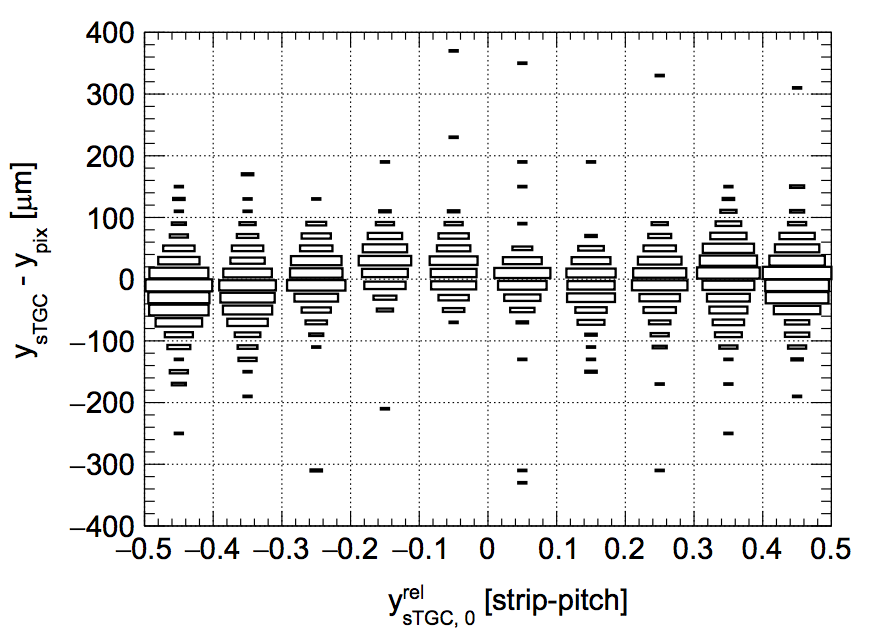
\includegraphics[width=\textwidth]{strip-aligned.png}
		\caption{The differential after sinusoidal correction is applied}\label{fig:pitchaligned}
	\end{subfigure}
	\hspace*{\fill}
	\caption{Charge distribution over strip-pitch}\label{fig:strip-pitch}
\end{figure}


The charge measured on the strips of the sTGC detector results from a spatial sampling and discretization of the induced
charge. The process of reconstructing the sTGC strip-cluster position from this sampling introduces a differential
non-linearity effect on the reconstructed strip-cluster position. \par

The deviation of the measured strip-cluster position from the expected position (estimated by the pixel telescope track)
depends on the strip-cluster position relative to the strips.  This dependence is clearly seen in the two dimensional
distributions in Figure \ref{fig:pitchfit}. It shows the y-residual versus strip-cluster position relative to the
closest inter-strip gap center $y_{\mathrm{sTGC},0}^{\mathrm{rel}}$. This effect is corrected using a sinusoidal
function:

	\begin{equation}\label{sin}
	 y_{\mathrm{sTGC}} = y_{\mathrm{sTGC},0}-a_i\sin \left(2\pi y_{\mathrm{sTGC},0}^{\mathrm{rel}}\right)
	\end{equation}
	
where $y_{\mathrm{sTGC},0}$ is the strip-cluster mean resulting from the Gaussian fit and $y_{\mathrm{sTGC}}$ is the
corrected particle position estimator. The amplitude parameters are denoted $a_i$ for the 3,4 and 5 strip-multiplicity
(cluster size). These amplitude parameters are free parameters in the fit. The values of the amplitude parameters
obtained from the fit to data are compatible with being equal for the three strip-cluster multiplicity as shown in Table
\ref{table}.\par

	\begin{table}
		\centering
		\caption{Fit parameters per cluster size}\label{table}
		\begin{tabular}{cc}
		\hline
		Strip-cluster multiplicity $i$ & Amplitude parameter $a_i$\\
		\hline
		3 & 205 $\pm$ 9\\
		4 & 206 $\pm$ 4\\
		5 & 211 $\pm$ 5\\
		\hline
		\end{tabular}
	\end{table}

The correction function is therefore universal and is shown in Figure \ref{fig:pitchfit}. The two dimensional
distribution after the correction is applied was found to be reasonably flat as shown in Figure
\ref{fig:pitchaligned}.\par

The alignment of the coordinate system of the pixel telescope with respect to the above-defined coordinate system of the
sTGC layer also affects the measured residual distribution. A simple two-parameter model is used to account for
translations and rotations of the two coordinate systems with respect to each other. Both the alignment correction and
the differential non-linearity correction are included {\it in situ} in the analysis. \par

The alignment correction is introduced in the model by expressing the pixel track position in the sTGC-layer coordinate
system $y_{\mathrm{pix}}$, as a function of the track position in the pixel telescope coordinate system
$x_{\mathrm{pix}}'$ and $y_{\mathrm{pix}}'$, and two misalignment parameters $\delta y$ and $\phi_{xy}$, as follows:

\begin{equation}
	y_{\mathrm{pix}}=-x_{\mathrm{pix}}' \sin \phi_{xy} + y_{\mathrm{pix}}'\cos \phi_{xy}+\delta y
	\end{equation}

The variable $\delta y$ corresponds to a misalignment along the y-axis of the sTGC coordinate system, and $\phi_{xy}$
corresponds to a rotation of the telescope coordinate system in the x-y plane around the z-axis of the sTGC coordinate
system. Translation and rotation misalignment along and around the other axis are not taken into account in this model,
since they are expected to have a small impact on the determination of the intrinsic position resolution.\par

	\begin{figure}[ht]
		\centering
		\hspace*{\fill}
		\begin{subfigure}[b]{0.42\textwidth}
			\centering
			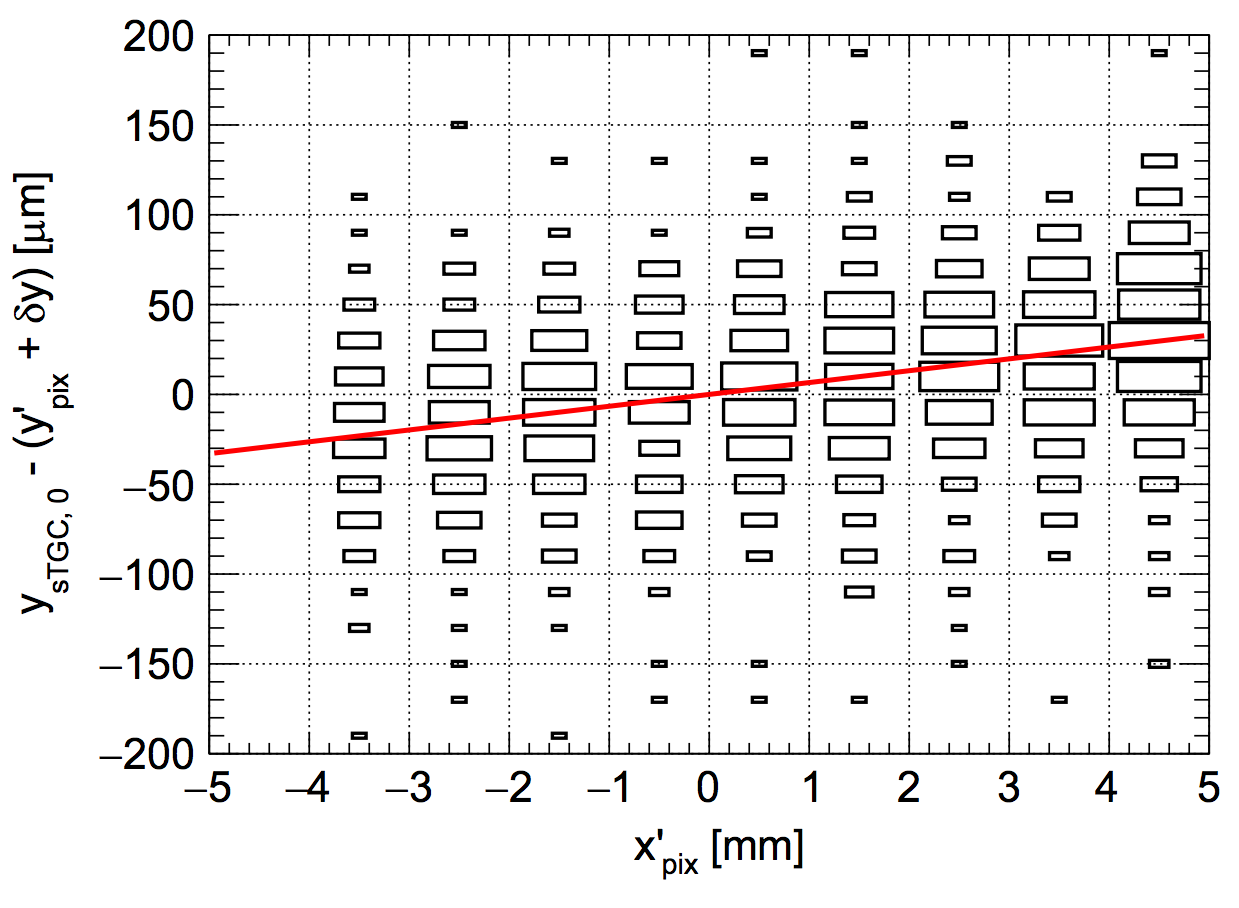
\includegraphics[width=\textwidth]{y-xplane.png}
			\caption{Residual y against x position on pixel telescope.}\label{xyplanefit}
		\end{subfigure}
		\hfill
		\begin{subfigure}[b]{0.42\textwidth}
			\centering
			\includegraphics[width=\textwidth]{y-xplanerotate.png}
			\caption{After rotation and translation applied}\label{xrotate}
		\end{subfigure}
		\hspace*{\fill}
		\caption{Coordinate system correction}\label{rotation}
	\end{figure}
	
	On the Figure \ref{xyplanefit} it is possible to observe the y-residual mean increase linearly as a function of the x
	position on the telescope called $x'_{\mathrm{pix}}$, which is evidence for a small rotation between the two
	coordinate systems. The red line represents the correction applied to this dataset. Accounting for this correction
	results in a distribution that is independent of $x'_{\mathrm{pix}}$ on Figure \ref{xrotate}.\par

 After all the corrections are applied, the calculations for the intrinsic resolutions are taken for each layer 
 and compared with  the residual distribution. A double Gaussian function (equation \ref{fit}) is fitted, where the first
 Gaussian represents the core of the residual distribution and the second one is a wider Gaussian which represents some
 reconstructed strip-cluster from background sources. \par
 
 \begin{eqnarray}
	F_i &=& F_i(y_{\mathrm{sTGC},0}, y_{\mathrm{sTGC},0}^{\mathrm{rel}}, x'_{\mathrm{pix}},y'_{\mathrm{pix}};\delta y,\phi_{xy},a_i,\sigma,f,\sigma_w)\\
			&=& f G(y_{\mathrm{sTGC}}-y_{\mathrm{pix}};0,\sigma) +
			(1-f)G(y_{\mathrm{sTGC}}-y_{\mathrm{pix}};0,\sigma_w)\label{fit}
	\end{eqnarray}


\begin{figure}[ht]
	\centering
	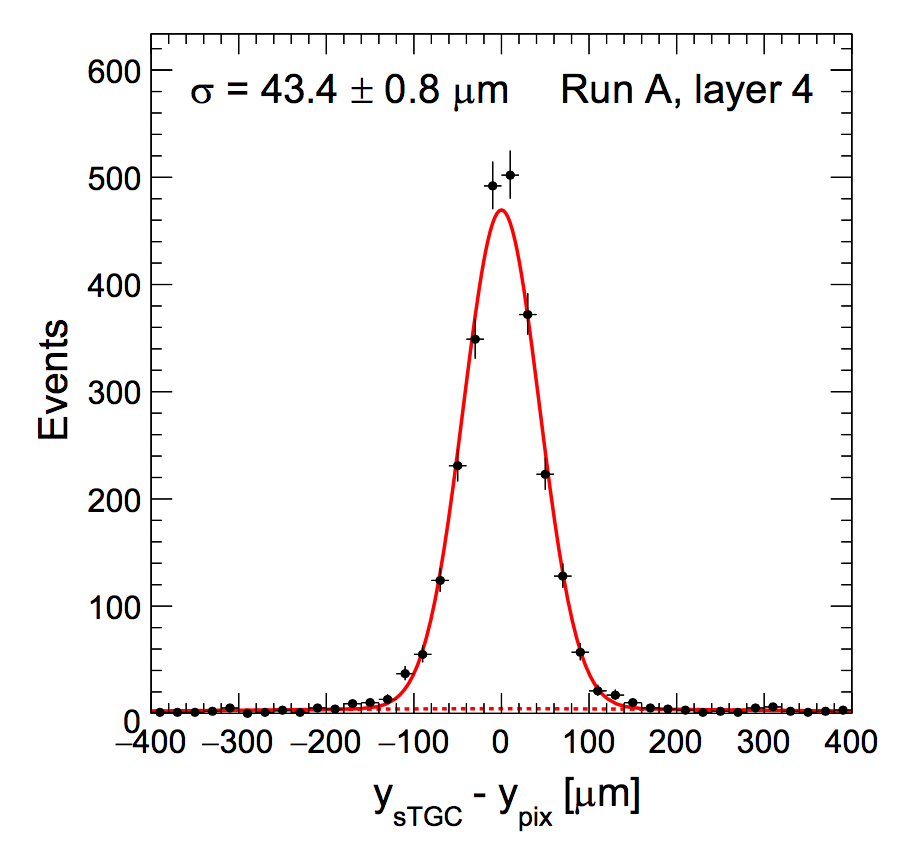
\includegraphics[width=0.4\textwidth]{resTelescope.png}
	\caption{Intrinsic resolution of layer 4, respect to pixel telescope.}\label{restelescope}
	\end{figure}

	\begin{figure}[ht]
	\centering
		\hspace*{\fill}
	\begin{subfigure}[b]{0.3\textwidth}
	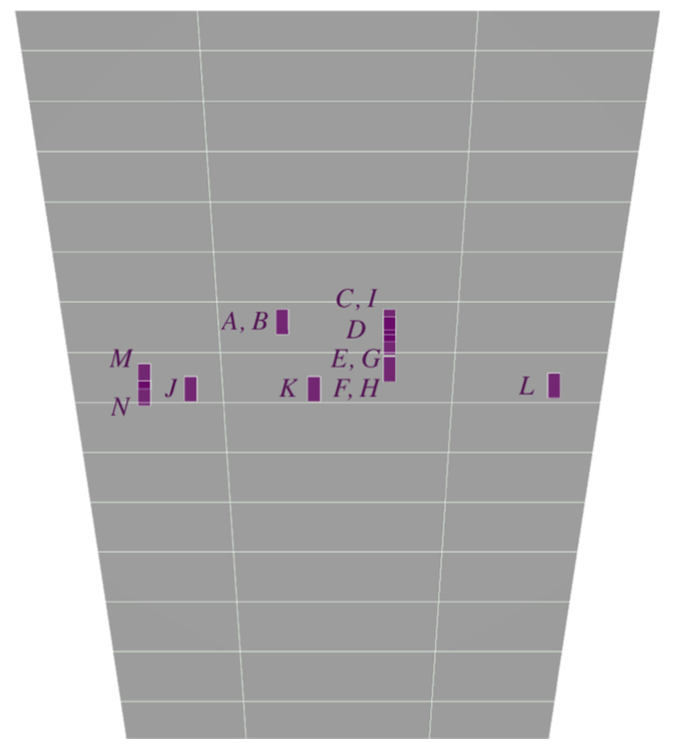
\includegraphics[width=\textwidth]{beampos.png}
	\caption{Beam position for different data sets on sTGC}\label{beampos}
	\end{subfigure}
	\hfill
	\begin{subfigure}[b]{0.45\textwidth}
	\centering
	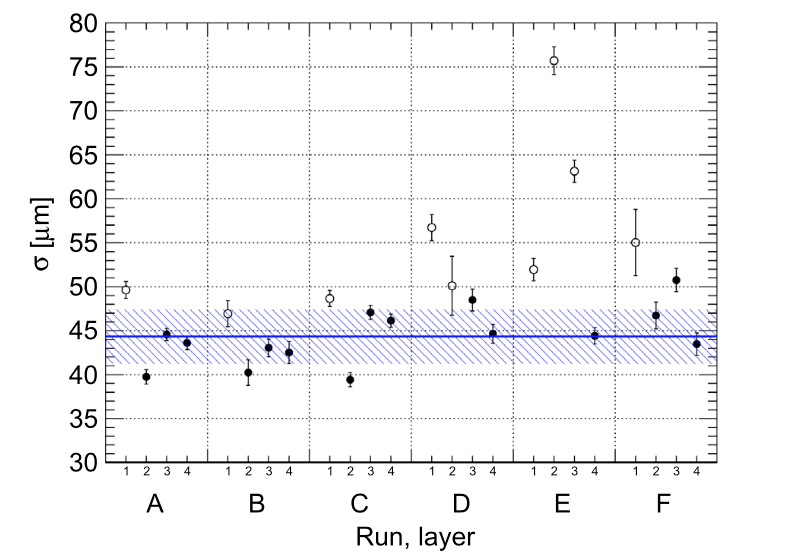
\includegraphics[width=\textwidth]{summaryTelescope.png}
	\caption{Summary of intrinsic resolution for each data set and layer of sTGC}\label{summary}
	\end{subfigure}
	\hspace*{\fill}
	\caption{Summary of pixel telescope analysis}\label{}
\end{figure}


On Figure \ref{restelescope} a set of events shows the distribution presented before with an intrinsic resolution
parameter $\sigma$ of about \unit{44}{\micro m} for a representative data taking run and sTGC strip-layer, where the red
line is the narrow Gaussian fit and the dashed line is the wider Gaussian fit.\par

The fraction of the data parameterized by the narrow Gaussian is around 95\% with a RMS of about 2\%.
The rest of data taking runs and its beam position can be observed on Figure \ref{summary}, where the black circles
represent the valid data and the open circles the runs with expected degradation due to detector structure supports or
individual channel pedestal.\par




	%----------------- STANDALONE ANALYSIS 	---------------


\subsubsection{sTGC standalone analysis}
\begin{figure}[ht]
\centering
\hspace*{\fill}
\begin{subfigure}[b]{0.45\textwidth}
\centering
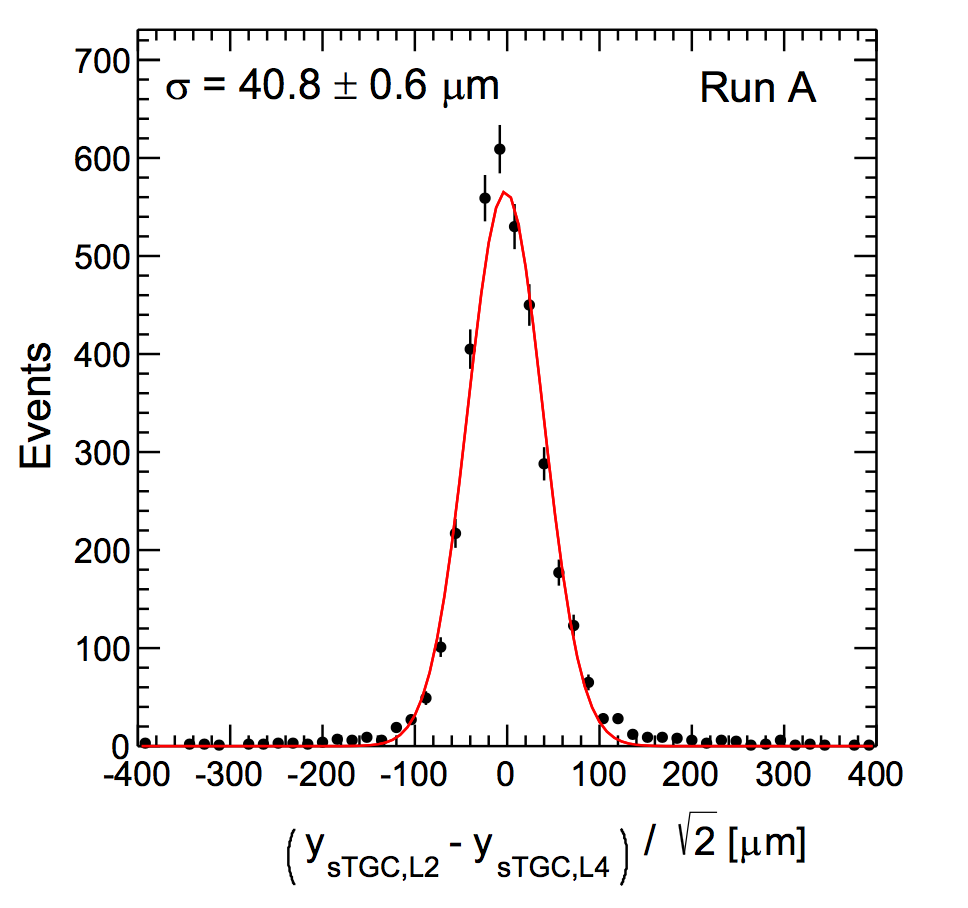
\includegraphics[width=\textwidth]{resStandalone.png}
\caption{}\label{pairwise}
\end{subfigure}
\begin{subfigure}[b]{0.45\textwidth}
\centering
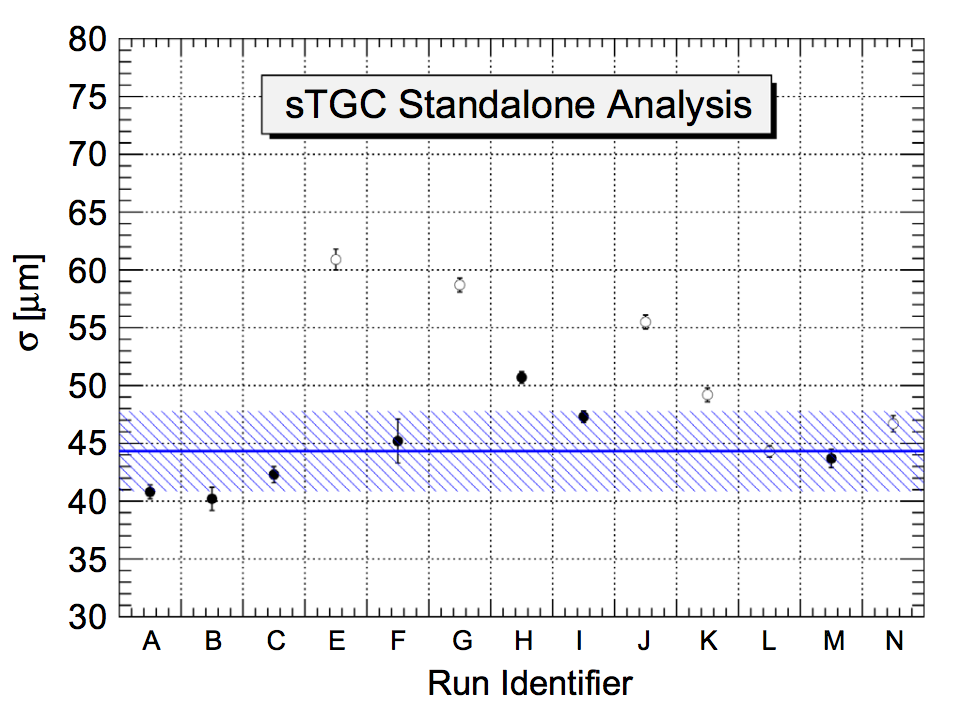
\includegraphics[width=\textwidth]{summaryStandalone.png}
\caption{}\label{sss}
\end{subfigure}
\hspace*{\fill}
		\captionsetup{margin=1cm}
\caption{(a) Resolution estimate based on adjacent sTGC strip-layer position residual distributions for a
representative sTGC standalone data taking run.\\
(b) Summary of the measured intrinsic sTGC resolution using the
pixel telescope analysis for different data taking runs. The beam position on the sTGC detector for each run is
shown in \ref{beampos}. Results for runs with no expected degradation due to sTGC detector support structure or
calibration are shown as black filled circles. The horizontal line represents the average resolution for these runs
whereas the hashed band represents the RMS spread.  Results for the remaining runs are shown as open circles. }\label{}

\end{figure}

In this analysis the correction for the differential non-linearity in respect to strip-pitch obtained before is kept,
however the residual distribution of the y-position is calculated from two pairwise layer of the sTGC.  Therefore half
of the variance of this distribution corresponds to our parameter to estimate the intrinsic resolution for one layer,
hence $\sigma = \sigma_{\mathrm{residual}}/\sqrt{2}$. \par
A strip-layer position residual distribution for a representative sTGC standalone data taking run is shown in Figure
\ref{pairwise}.\\ In this graph, a intrinsic resolution of $\sigma=40.8\pm0.8\mu m$ is obtained.

In summary of fourteen data sets, the intrinsic resolution with this analysis is about \unit{45}{\micro m}. The white
open circles on the graph \ref{sss} correspond to non-validate data due to wire-support position or mis-calibrations.
The hash band represents the RMS spread and the blue line is the average.\par 



\section{Pad efficiency}\label{padeff}

One of the new features of the small-strip Thin Gap Chamber compare to its previous version is the possibility to
provide a fast trigger for the Region of Interest from the \unit[8x50]{cm$^2$} pad area, where 3 out of 4 pads from a
sTGC quadruplet can confirm a particle candidate, therefore a track position can be obtained from the strips within this
area.\par

A test beam experiment was conducted at the CERN H6 beam line, using a \unit[130]{GeV} muon beam of about \unit[4]{cm}
radius, a wider beam spot to test the characteristics of the pads. The setup is shown in Figure \ref{padsetup} where the
system was triggered by a set of scintillators (in blue) with a \unit[12x12]{cm$^2$} coincidence area.\par

As explained before, for the beam tests a preliminary front-end electronics based on the VMM1 was used. This ASIC
provides a Time-over-Threshold (ToT) signal as digital output, however is also possible to get a analog pulses.  During the
test beam, using the present configuration, an inefficiency was observed related to small late charges from the sTGC
detector which may be not well adapted to the VMM1. An efficiency of 80-90\% was observed running at
\unit[100]{kHz/cm$^2$}.\par


\begin{figure}[ht]
\centering
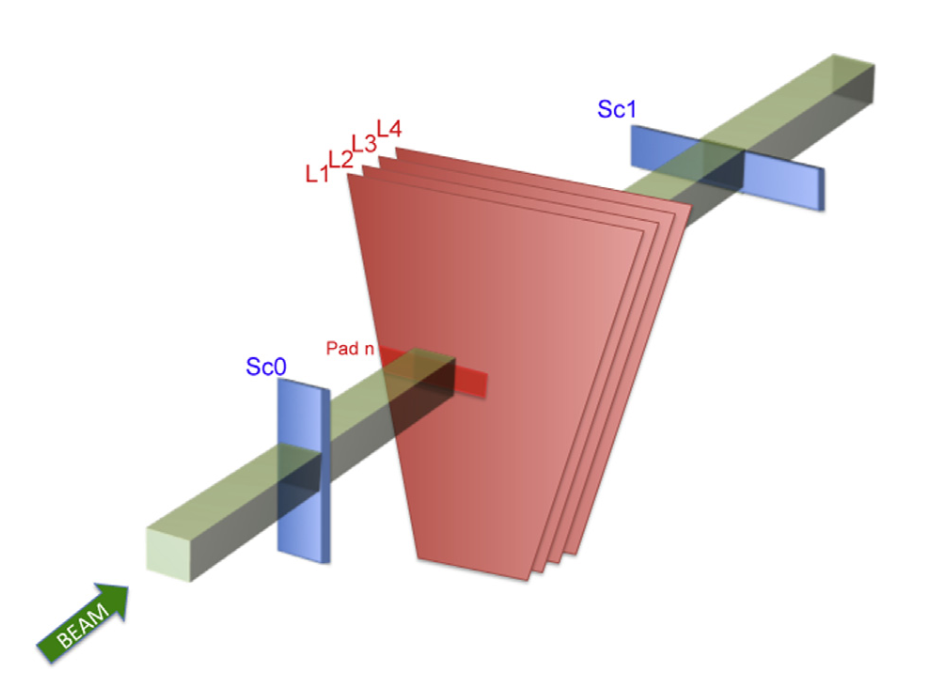
\includegraphics[width=0.6 \textwidth]{padSetup.png}
\caption{Setup for pad measurements. Coincidence block in  light green. Pad $n$ in red. Scintillators in blue.}\label{padsetup}
\end{figure}


To ensure that no inefficiency was due to the detector itself, the large cathode pads were used to estimate the detector
efficiency, which was measured by looking at the analog output of the front-end amplifier. The efficiency of the pad $n$
in the first layer was defined with respect to the coincidence of the trigger with a signal in the fully overlapping pad
of the second layer. \par



\begin{figure}[t]
\centering
\hspace*{\fill}
\begin{subfigure}[b]{0.45\textwidth}
\centering
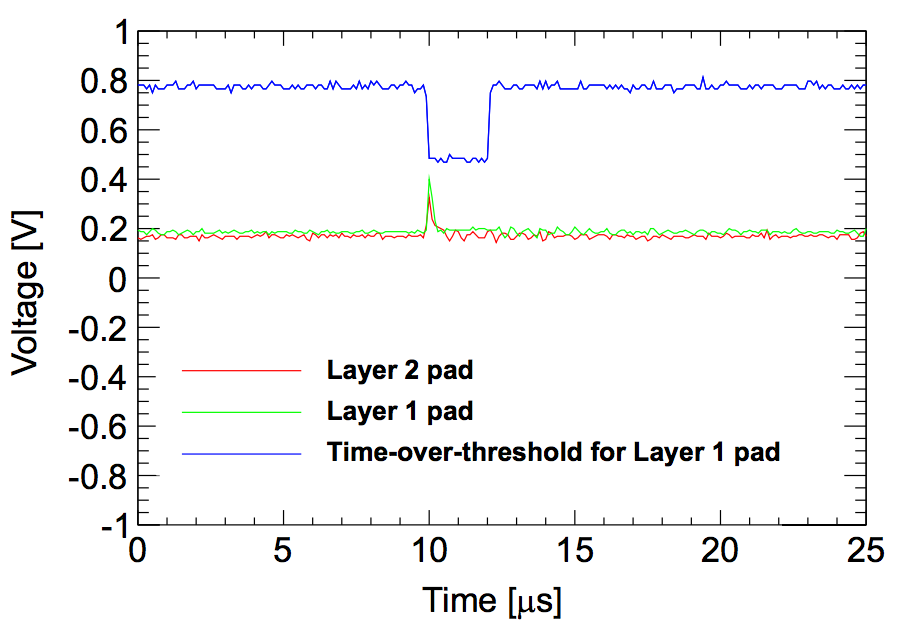
\includegraphics[width=\textwidth]{padnormal.png}
\caption{ToT signal from pad L1, pad L2 as a trigger}\label{scope1}
\end{subfigure}
\hfill
\begin{subfigure}[b]{0.45\textwidth}
\centering
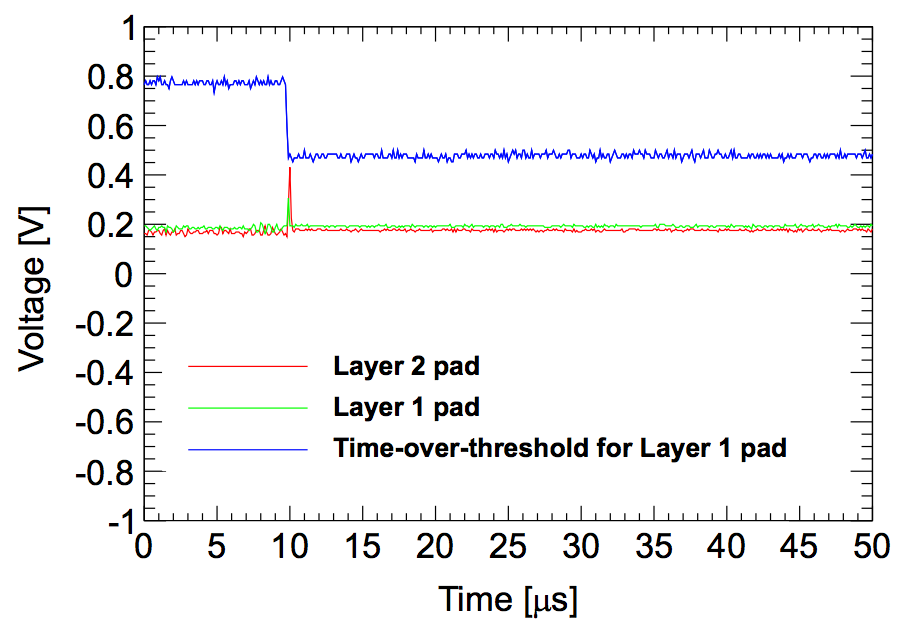
\includegraphics[width=\textwidth]{paddeadtime.png}
\caption{Large dead time on ToT signal from pad L1}\label{scope2}
\end{subfigure}
\hspace*{\fill}
\caption{Digital and analog signal from VMM1}\label{scope}
\end{figure}

Two examples from this configuration are shown on Figure \ref{scope}; on the left a two analog signals from pads are
present with a ToT signal from layer 1 with about 2 \micro s length, meanwhile on the right picture a long ToT pulse
with more than 40 \micro s length when the two analog signal are present. By recording hundreds of triggered events
using an oscilloscope, the presence of a detector signal within the live-part of the front-end electronics (independent
of the signal threshold) was checked. This test confirmed that the detector was 100\% efficient.\par


\subsubsection{Charge sharing between pads}


To study the transition region between pads, the scintillator coincidence triggering area and the particle beam were
centered between pad $n$ and pad $n+1$ of the first layer, as illustrated in Figure \ref{chargepos}.\par

After applying timing quality requirements on the strip and pad hits, the channel baseline values are subtracted from
the analog peak values. Strip-clusters with induced charge in either 3,4 or 5 adjacent strips are selected and
calibrated in the same way as for the Fermilab beam test.\par

Events with a single strip-cluster in the first layer and the second layer are selected. The strip-cluster position
(mean of the fitted Gaussian) in the first layer is used to define the position of the particle going through the
detector. The events are further required to contain a hit above threshold on either pad $n$ or pad $n+1$. The charge
fraction ($F$) is defined using the analog peak values ($P$) of the two adjacent pads:

\begin{equation}
F = \frac{P_n - P_{n+1}}{P_n + P_{n+1}}
\end{equation}

\begin{figure}[H]
\centering
\hspace*{\fill}
\begin{subfigure}[b]{0.45\textwidth}
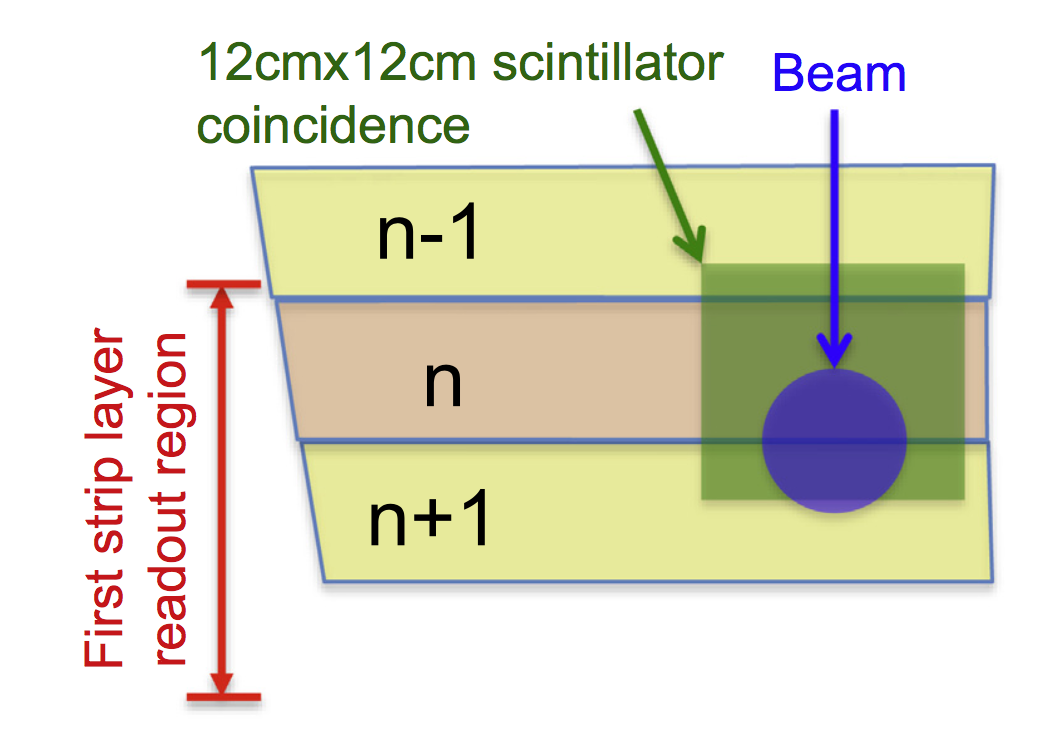
\includegraphics[width=\textwidth]{chargepos.png}
\caption{Pad region transition scheme}\label{chargepos}
\end{subfigure}
\hfill
\begin{subfigure}[b]{0.45\textwidth}
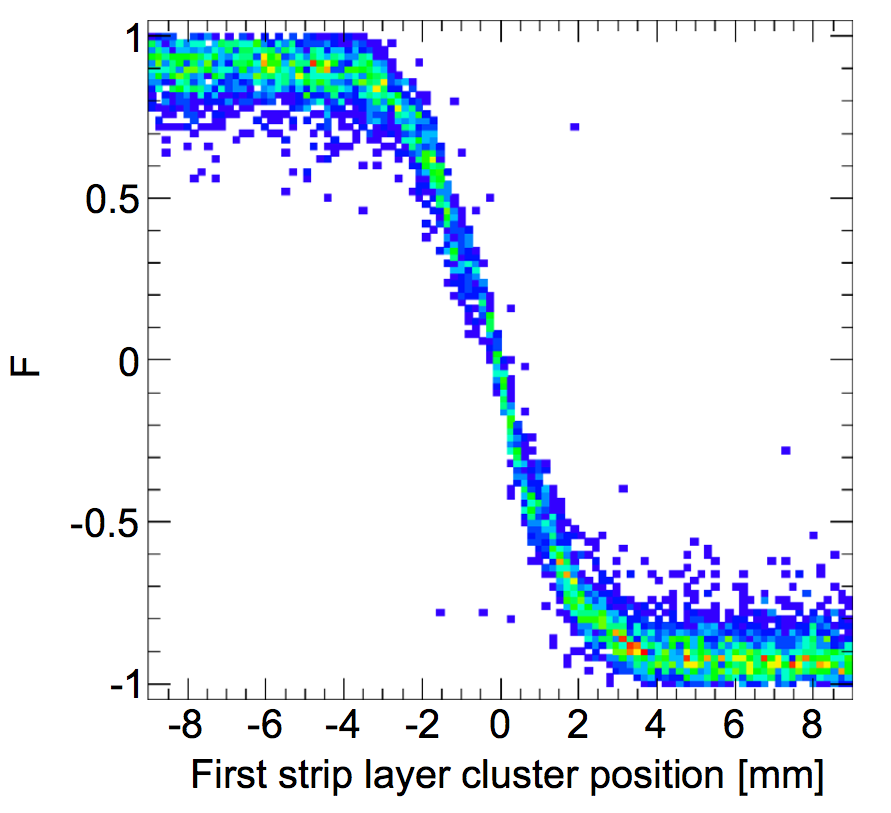
\includegraphics[width=\textwidth]{chargeSharing.png}
\caption{Charge Sharing distribution}\label{chargeSharing}
\hspace*{\fill}
\end{subfigure}
\caption{}\label{}
\end{figure}


Figure \ref{chargeSharing} shows the charge fraction as a function of the position with respect to the center of the
transition region, where the two pads share more than 70\% of the induced charge, spans about \unit{4}{mm}.\par

\section{Summary}

In the chapter we introduce the construction process and discuss the phenomenology of the sTGC. The main features of
this Thin Gap Chamber are presented. The smaller strips of 3.2mm pitch give the spatial resolution needed for the
improvement of the New Small Wheel of ATLAS. The main problem to achieve this precise 3.2mm$\pm$50\micro m pitch in long
boards (1m to 2m long) is discussed.\par
To improve the time response the resistivity of the graphite layer is decreased and the distance between the readout and
graphite layer is reduced to a 100\micro m.\par

The sTGC detector is tested with four different objectives. The first test under x-rays occurs right after the Quadruplet is
constructed. The use of this source helps to understand the construction issues as well as qualifying process, where
the uniformity of the gain is measured.\par

Certainly, multiple factors can be improved in this test, such as increasing the vertical and horizontal steps to benefit from the 2mm spot size of the x-ray gun. 
Although the entire process for this test can be improved, the Module\#0 shows an overall 17\% uniformity for the four
chambers.\par

In the Section \ref{gifff} a direct measurement of the rate in a high irradiation environment is provided by a small size
sTGC. The references values obtained help to set a working point to test the new Quadruplets against high flow rate.
The non-linear change in the resistivity of the chamber for different particles rates suggests a better election for the
resistor component connected to the anode wires. All the group wires are connected in series to a \SI{10}{M\Omega},
however, not all the groups receive the same amount of charge in an homogeneous particle rate because of the different
lengths in the trapezoidal shape of the sTGC. \par

The last two sections summarize the two test beams for the first sTGC prototype, where crucial results are obtained for
the electronics in charge of the readout. The test beam in CERN helps to understand the inefficiency of the Pads.
The electronics designed for this detector (VMM1) has some issues which provides a 80-90\% efficiency running at
\SI{100}{kHz/\cm^2}. The detector is discarded, therefore, the VMM1 needs to be improved. \par

On the sTGC technology, all the efforts go to the improvement of the position resolution and the Section
\ref{resolution} shows a intrinsic resolution of about \SI{40}{\micro m} for the standalone analysis.\par

The spatial resolutions and pad efficiency results have been published in ``Performance of a full-size small-strip thin gap chamber prototype
for the ATLAS new small wheel muon upgrade''\cite{performance}.

The estimation of the position and efficiency resolution as a function of background rates inside the high rate
environmental with a muon beam is remaining and it will be done after a new version of the VMM1 electronics is produced.  
